\documentclass[12pt, letterpaper]{article}

% Packages
\usepackage[utf8]{inputenc}
\usepackage[T1]{fontenc}
\usepackage{amsmath, amssymb, amsfonts}
\usepackage{graphicx}
\usepackage{booktabs}
\usepackage{hyperref}
\usepackage[margin=1in]{geometry}
\usepackage{float}
\usepackage{enumitem}
\usepackage{caption}
\usepackage{subcaption}
\usepackage{algorithm}
\usepackage{algpseudocode}
\usepackage{natbib}
\usepackage{setspace}
\usepackage{fancyhdr}
\usepackage{multirow}
\usepackage{longtable}

\graphicspath{{outputs/figures/}}

\doublespacing

\pagestyle{fancy}
\fancyhf{}
\rhead{CPE 595 -- Machine Learning}
\lhead{Asset Cluster Migration}
\rfoot{Page \thepage}

\begin{document}
\thispagestyle{empty}

\begin{center}
{\Large \textbf{Dynamic Multi-Layer Asset Topology and}}\\[0.3em]
{\Large \textbf{Cluster Migration Under Geopolitical Stress}}\\[0.8em]
{\normalsize A Regime-Aware Framework for Detecting Structural Breaks in Cross-Asset\\Dependency Networks}\\[1.5em]
{\normalsize Nicholas Tavares \hspace{1.5em} Amjad Hanini \hspace{1.5em} Brandon DaSilva}\\[1.2em]
{\normalsize \textit{CPE 595 -- Machine Learning}}\\[0.2em]
{\normalsize \textit{Professor Shucheng Yu}}\\[0.2em]
{\normalsize \textit{Stevens Institute of Technology}}\\[0.8em]
{\normalsize March 2026}
\end{center}
\vspace{0.5em}

\begin{abstract}
This paper presents a dynamic multi-layer network framework we developed for tracking how global asset relationships reorganize during periods of geopolitical stress. The motivation came from a straightforward observation: traditional correlation-based analysis consistently fails to capture what is actually happening in markets when a crisis unfolds. Rather than relying on a single correlation matrix, our approach constructs three parallel dependency layers (linear shrinkage correlation, nonlinear distance correlation, and empirical tail co-exceedance), applies Leiden community detection over rolling windows, and introduces two novel quantitative metrics for measuring structural change. The first is a permutation-invariant Cluster Migration Index (CMI) built on Hungarian matching, and the second is a z-score normalized Topology Deformation Score (TDS) that fuses degree distribution shifts, community divergence, and spectral distance into a single composite. On top of this, we implemented transfer entropy and Granger causality to determine directional information flow between assets across different market regimes. Running the full pipeline on a 96-ETF universe covering equities, fixed income, commodities, currencies, crypto, managed futures, and 18 country-specific funds from January 2010 through March 2026, one pattern kept appearing across every event window we studied: markets begin restructuring \textit{before} the geopolitical event, not during it. Tail dependence picks up the signal first. Correlation catches up later.
\end{abstract}

\newpage
\tableofcontents
\newpage

%----------------------------------------------------------------------
\section{Introduction}
%----------------------------------------------------------------------

Most cross-asset analysis boils down to some variation of a correlation matrix. Compute pairwise Pearson correlations, maybe visualize it as a heatmap, and that is more or less the standard playbook. The issue with this is pretty fundamental: correlation is a linear measure, and markets do not break down in linear ways.

Take COVID as an example. Correlations across the board shot up to nearly 1.0 for a brief stretch, then reverted almost as quickly. Everything moved together, then stopped moving together. On the surface that looks like a temporary shock with no lasting structural change. But when we actually examined the community structure of the asset network through that period, we found something different: every single asset changed its cluster assignment. The entire topology dissolved and reformed. A Pearson heatmap does not tell you that story.

Then look at the Iran-Israel escalation cycle in 2024-2025. Pearson correlation barely flinched during some of these events. If that was your only lens, you would have concluded nothing structurally interesting happened. But the nonlinear and tail-dependence layers told a completely different story, with massive restructuring happening underneath the surface that linear correlation was blind to.

These observations are what pushed us to build this framework. We had a few questions we wanted to answer:

\begin{enumerate}[label=\arabic*.]
    \item Do asset clusters genuinely restructure during geopolitical events, or does everything just co-move temporarily and snap back?
    \item Is it possible to detect that restructuring \textit{before} the event actually hits, using dependency measures beyond standard correlation?
    \item Does structural change propagate in a specific causal direction across different dependency layers?
    \item Which assets sit at the boundaries between clusters and serve as contagion pathways during stress?
\end{enumerate}

Our methodology combines graph-based community detection (Leiden algorithm), unsupervised regime learning (Gaussian Hidden Markov Models), information-theoretic causality (transfer entropy), and classical hypothesis testing (Granger causality) into a unified pipeline. We introduce permutation-invariant migration metrics built on the Hungarian algorithm, and validate everything with bootstrap confidence intervals, surrogate null distributions, and walk-forward out-of-sample testing.

The label permutation problem alone was introducing so much noise into the existing literature's migration measurements that we felt it warranted a ground-up rethinking of how these metrics should be computed. So we did that, built the full pipeline from data ingestion through topology export, and ran it across 16 years of daily data spanning 8 major geopolitical events.

%----------------------------------------------------------------------
\section{Related Work}
%----------------------------------------------------------------------

The idea of applying network theory to financial markets goes back to Mantegna \cite{mantegna1999}, who showed that minimum spanning trees built from correlation matrices reveal hierarchical clustering in equity markets. Tumminello et al. \cite{tumminello2005} extended this with the Planar Maximally Filtered Graph (PMFG), which preserves richer topological information than MSTs while still filtering out noise. Both of these are foundational to our graph construction layer.

On the community detection side, the Louvain algorithm was the standard for years, but Traag et al. \cite{traag2019} demonstrated that Louvain can produce disconnected communities and introduced Leiden as a replacement with guaranteed connectivity. We use Leiden as our primary clustering method for this reason. The application of community detection to financial networks has been explored by several groups, but most of this work operates on static or slowly-rolling single-layer correlation matrices. MacMahon and Garlaschelli (2015) applied stochastic block models to financial correlation networks, and Musmeci et al. (2015) used filtered graphs with Louvain on rolling windows. Neither addresses the label permutation problem that contaminates temporal cluster comparisons.

Multi-layer network analysis in finance is more recent. Musmeci et al. (2017) built multiplex networks from Pearson and partial correlations, showing that different layers capture different market dynamics. Our approach extends this to three layers (linear, nonlinear, and tail) and adds cross-layer agreement tracking as a meta-signal.

For regime detection, Hamilton's (1989) seminal work on Markov switching models established the framework we build on. We use Gaussian HMMs following Rabiner (1989), but trained on a topology-derived state vector (realized volatility, mean correlation, dispersion) rather than raw asset returns, which is a departure from the standard approach in the regime detection literature.

Transfer entropy as a measure of directed information flow in financial systems has been explored by Marschinski and Kantz (2002) and more recently by Dimpfl and Peter (2013), who applied it to stock market indices. The KSG $k$-nearest-neighbor estimator \cite{kraskov2004} gives us a nonparametric estimate that avoids binning artifacts. Our contribution here is applying TE in a regime-conditional framework and demonstrating cross-layer Granger causality between tail-dependence CMI and Pearson CMI.

The Hungarian algorithm \cite{kuhn1955} for optimal assignment is well-established in combinatorial optimization, but to our knowledge it has not been applied to the cluster label matching problem in rolling financial network analysis. This is one of our primary methodological contributions.

On the robustness side, Politis and Romano \cite{politis1992} established the block bootstrap for dependent data, and Theiler et al. \cite{theiler1992} introduced surrogate data testing for nonlinearity. Schreiber and Schmitz \cite{schreiber1996} improved on this with IAAFT surrogates. We apply all three in our validation framework, along with Benjamini-Hochberg \cite{benjamini1995} and Storey \cite{storey2002} corrections for the multiple testing burden inherent in pairwise causality analysis across 96 assets.

%----------------------------------------------------------------------
\section{Description of the Dataset}
%----------------------------------------------------------------------

\subsection{Asset Universe and Data Source}

Our universe consists of 96 ETFs, selected specifically for cross-asset breadth. The whole point of studying cluster migration is to see assets move between structurally different groups, so if you populate your universe with 96 flavors of US large-cap equity, you will not learn much. We needed genuine diversity: Treasuries that rally on flight-to-safety flows, commodities that respond to supply disruptions, EM currencies that get crushed during dollar strength, and so on.

\begin{table}[H]
\centering
\caption{Asset Universe Composition (96 ETFs)}
\begin{tabular}{@{}lrl@{}}
\toprule
\textbf{Category} & \textbf{Count} & \textbf{Examples} \\
\midrule
US Equity \& Value & 9 & SPY, QQQ, IWM, DIA, VTI, SCHD \\
US Sectors & 13 & XLE, XLF, XLV, XLK, XLU, SOXX \\
International Equity & 8 & EFA, EEM, FXI, EWZ, EWJ \\
Country ETFs & 18 & EIS, INDA, EWG, EWT, ARGT, COLO \\
Fixed Income & 8 & TLT, IEF, SHY, LQD, HYG, EMB \\
Commodities & 10 & GLD, SLV, USO, DBA, URA, COPX \\
FX \& Volatility & 4 & UUP, FXE, FXY, VIXY \\
Thematic \& Defense & 4 & ITA, XAR, QTUM, BLOK \\
Global X Thematic & 16 & BOTZ, LIT, AIQ, BUG, CLOU \\
Managed Futures & 4 & DBMF, KMLM, CTA, WTMF \\
Crypto & 2 & BITO, IBIT \\
\bottomrule
\end{tabular}
\end{table}

The 18 country-specific ETFs were especially critical for our geopolitical event studies. Having EIS (Israel) in the universe lets us directly observe how the Israeli equity market repositions relative to global clusters during the Iran-Israel conflict cycle. Same logic for INDA, EWG, EWT, and the others.

All data comes from the Financial Modeling Prep (FMP) API on their Ultimate tier plan. FMP is a financial data provider that offers institutional-grade market data through a REST API, covering equities, ETFs, fixed income, economic indicators, and more. We use their stable endpoint (\texttt{historical-price-eod/dividend-adjusted}) which returns dividend-adjusted daily closing prices going back to each ETF's inception date. The Ultimate plan gives us up to 3,000 API calls per minute and 150 GB of bandwidth, which is more than enough to fetch and maintain the full 96-ticker universe with room to scale. Our client implements async HTTP requests with a token-bucket rate limiter, parquet-based caching so we only re-fetch stale data (anything older than one business day), and automatic retry with exponential backoff.

\subsection{Preprocessing Pipeline}

The raw data goes through several cleaning steps before anything else touches it. We compute log returns and apply 1\% Winsorization to handle extreme outliers without removing them entirely. Forward-fill handles gaps up to 5 trading days (holidays, exchange closures), and any ETF with more than 5\% of its data missing gets automatically excluded from that particular rolling window.

Out of the 96 ETFs in the universe, 59 survived the full cleaning process across the entire 16-year sample. The other 37 are newer funds (things like IBIT, which launched in January 2024, or SHLD from March 2024) that simply do not have enough history for the earlier rolling windows. They get included automatically once they accumulate sufficient data.

The final dataset covers 3,938 trading days from January 2010 through March 2026, producing 764 rolling windows at a 120-day width with a 5-day step.

\subsection{Data Visualization and Insights}

To get a sense of the raw dependency structure, Figure~\ref{fig:corr_heatmap} shows the full-sample Ledoit-Wolf shrinkage correlation matrix ordered by asset class. A few things jump out immediately. US equities (top-left block) are tightly correlated with each other, which is expected. Fixed income (TLT, IEF, SHY) is negatively correlated with equities, also expected. But look at the commodity block (GLD, SLV, USO, DBA): the correlations are much weaker and more heterogeneous. These are the assets that sit at the cluster boundaries and migrate most frequently.

\begin{figure}[H]
\centering
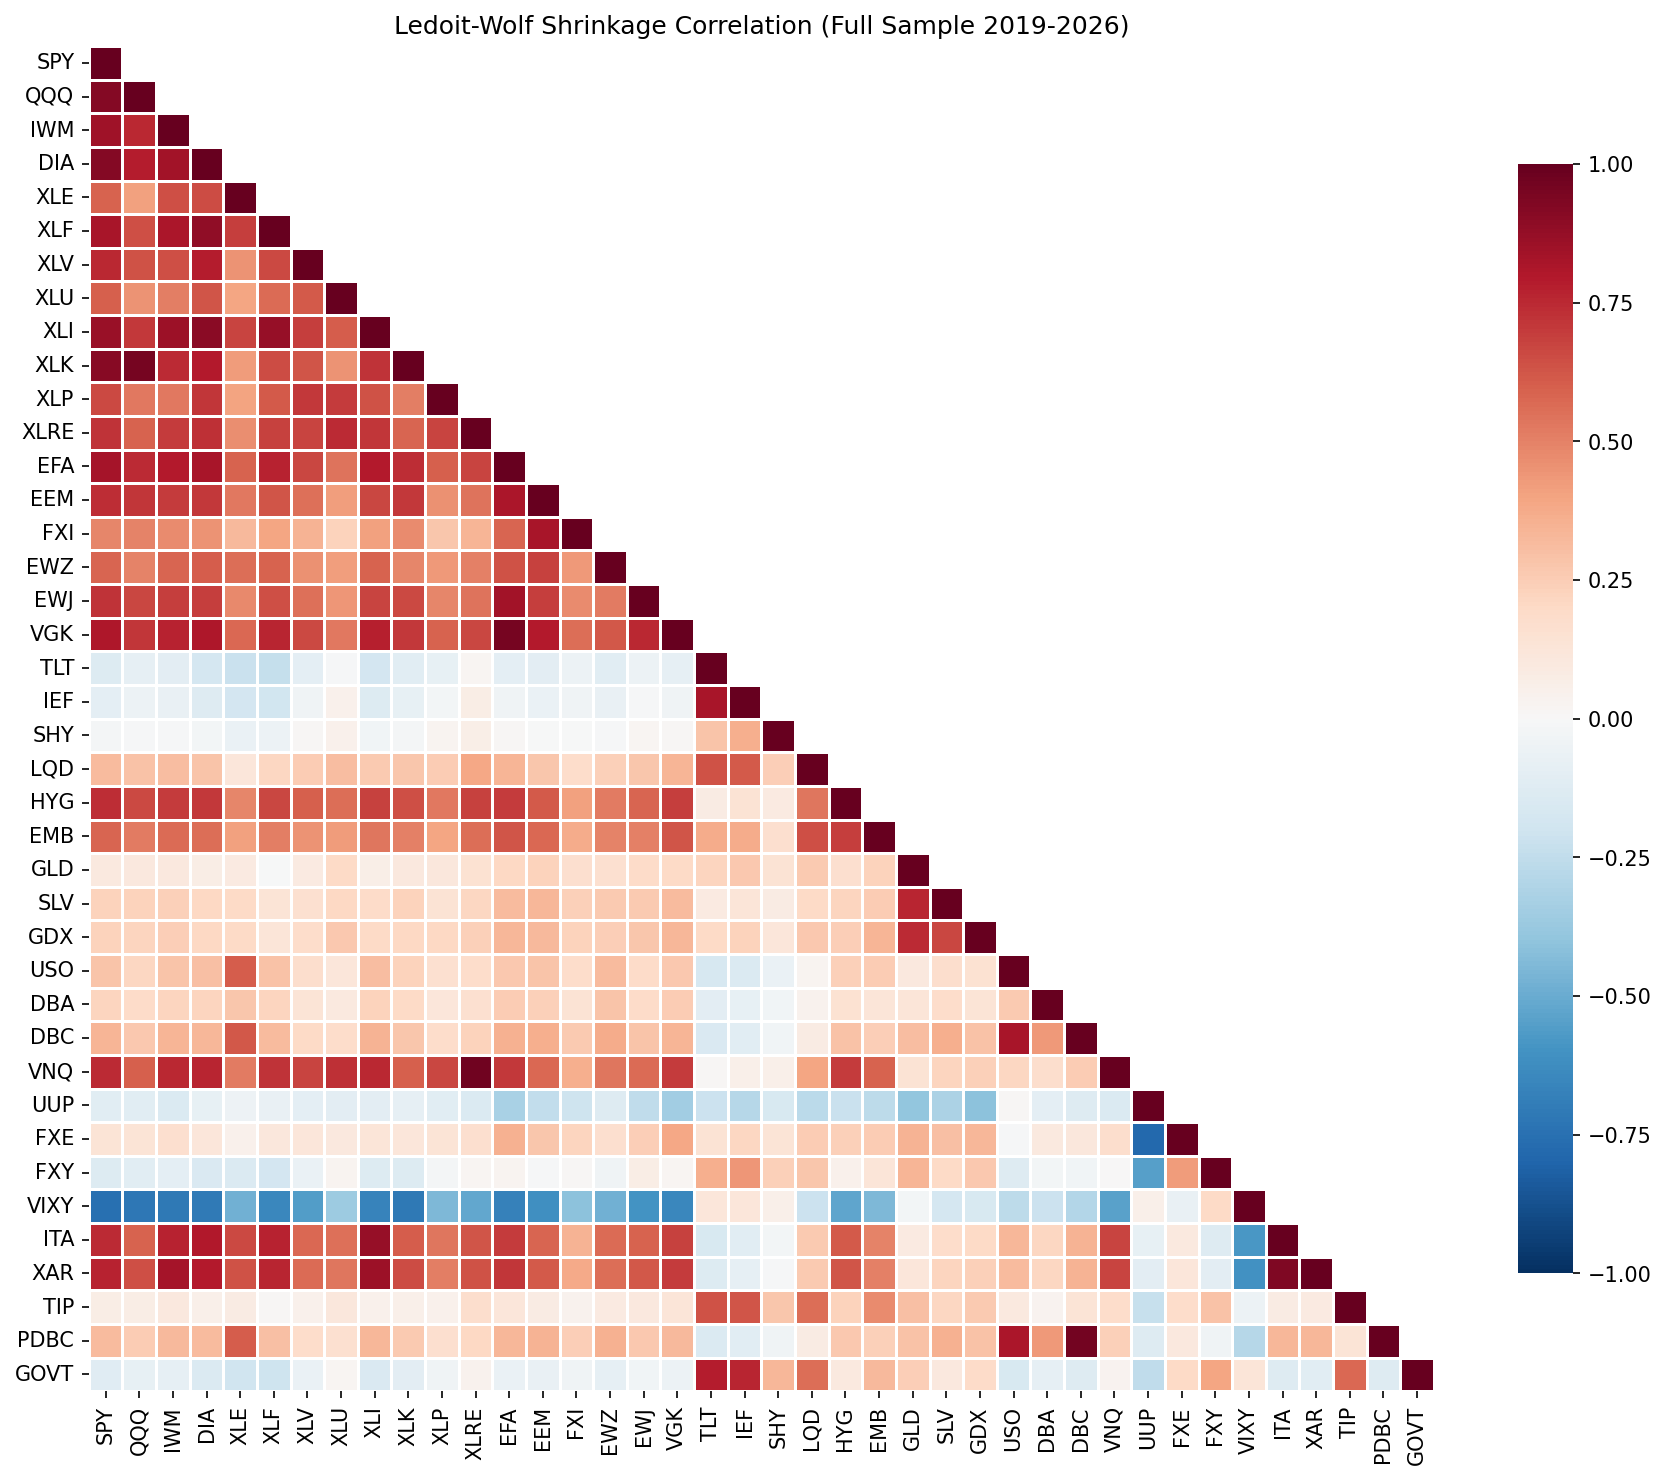
\includegraphics[width=0.85\textwidth]{fig3_correlation_heatmap.png}
\caption{Ledoit-Wolf shrinkage correlation matrix across the full sample period. The block-diagonal structure reveals natural asset groupings, while off-diagonal patterns (e.g., VIXY's strong negative correlation with equities) highlight the cross-asset dependencies that drive cluster formation.}
\label{fig:corr_heatmap}
\end{figure}

Figure~\ref{fig:multilayer_cmi} shows the per-layer Cluster Migration Index over time for all three dependency layers. This is one of the most revealing visualizations in the project. The three panels show CMI computed independently on the Pearson (blue), distance correlation (green), and tail-dependence (red) layers. Notice how different the three layers behave: during the 2025 geopolitical events, the tail-dependence layer shows sustained elevated CMI while the Pearson layer stays relatively flat. This is the multi-layer divergence that motivated the entire framework.

\begin{figure}[H]
\centering
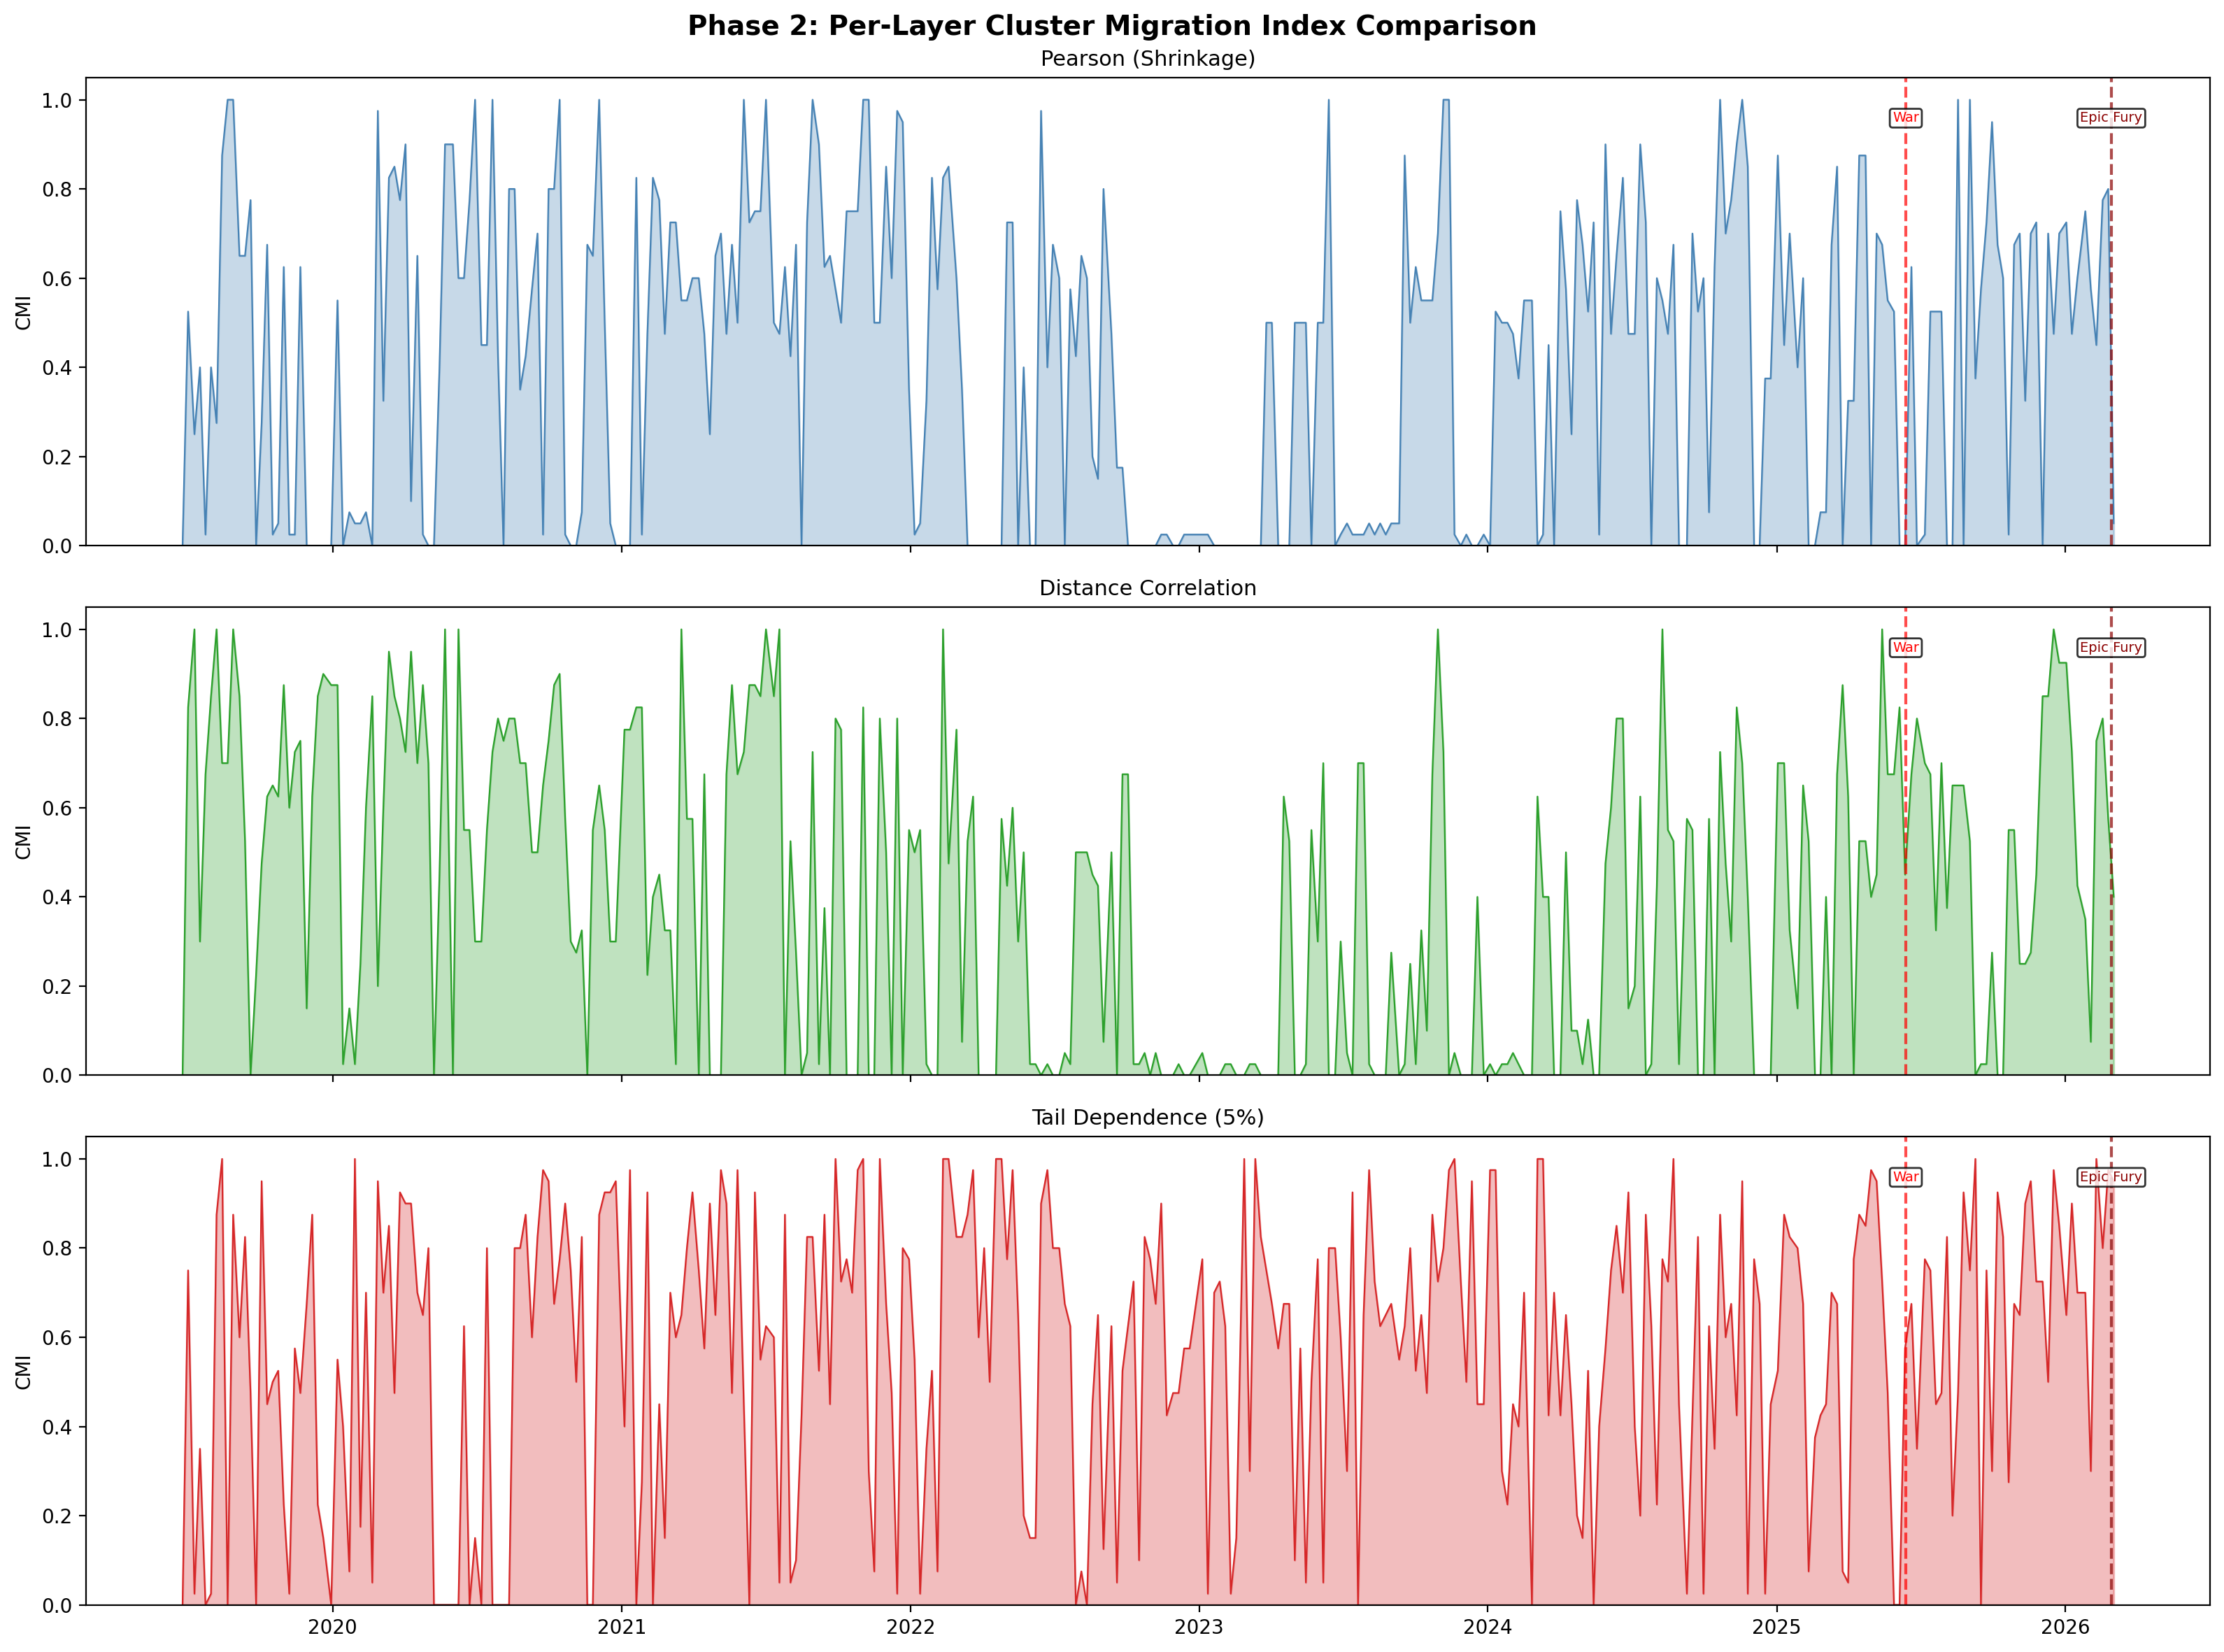
\includegraphics[width=\textwidth]{fig8_multilayer_cmi_comparison.png}
\caption{Per-layer CMI comparison across Pearson (top), distance correlation (middle), and tail dependence (bottom). The three layers respond differently to the same events, with tail dependence often leading structural change.}
\label{fig:multilayer_cmi}
\end{figure}

%----------------------------------------------------------------------
\section{Machine Learning Algorithms}
%----------------------------------------------------------------------

The framework relies on four distinct machine learning algorithms, each chosen for a specific role in the pipeline. We deliberately avoided using a single monolithic model and instead combined specialized methods that each handle one aspect of the problem well.

\subsection{Leiden Community Detection (Unsupervised Graph Clustering)}

Leiden \cite{traag2019} is a graph-based community detection algorithm that partitions nodes into groups by optimizing a modularity objective. It is the successor to the widely-used Louvain algorithm and fixes a known issue where Louvain can produce disconnected communities. For our problem, Leiden is the right choice because we are not trying to cluster assets in feature space (which is what K-Means does). We are trying to find communities in a dependency \textit{graph}, where edges represent the strength of pairwise relationships. Graph-based clustering naturally captures the network structure that feature-space methods ignore.

We run Leiden on each of the three dependency layers independently, then combine results through multiplex consensus. A resolution parameter controls the granularity of the clustering (higher resolution = more, smaller clusters), and we sweep it from 0.3 to 2.0 in our sensitivity analysis.

\subsection{K-Means Clustering (Baseline Comparison)}

We implemented K-Means as a baseline specifically to show what a standard feature-space clustering method misses. K-Means operates on the correlation matrix directly, treating each row as a feature vector and grouping assets by Euclidean distance in correlation space. It is fast and well-understood, but it has no concept of graph topology. It cannot distinguish between an asset that is weakly connected to everything and an asset that is strongly connected to a specific subgroup.

We run K-Means on the exact same rolling windows as Leiden and compare per-window results using Adjusted Rand Index (ARI), Normalized Mutual Information (NMI), and silhouette scores. This gives us a quantitative measure of how much structural information the graph-based approach captures beyond what K-Means can see.

\subsection{Gaussian Hidden Markov Model (Regime Detection)}

The 3-state Gaussian HMM is how we identify what market regime the system is in at any given point. The model treats the observable topology state vector (realized volatility, mean pairwise correlation, cross-sectional return dispersion) as emissions from one of three hidden states, and learns the transition probabilities between states from the data.

Why HMM over simpler threshold-based regime classification? Because regime boundaries are not clean. There is no single volatility level where you can draw a line and say ``above this is stress, below is calm.'' The HMM handles this by learning a probabilistic model of how the system transitions between states, assigning each window a probability distribution over regimes rather than a hard label. The three states auto-order by volatility: calm (89.7\% of windows), transition (5.1\%), and stress (5.2\%).

Figure~\ref{fig:regime_detection} shows the HMM regime labels overlaid on the topology state vector. The stress regimes (red shading) align closely with known crisis periods: COVID in early 2020, the Fed hiking cycle in late 2022, and the current period.

\begin{figure}[H]
\centering
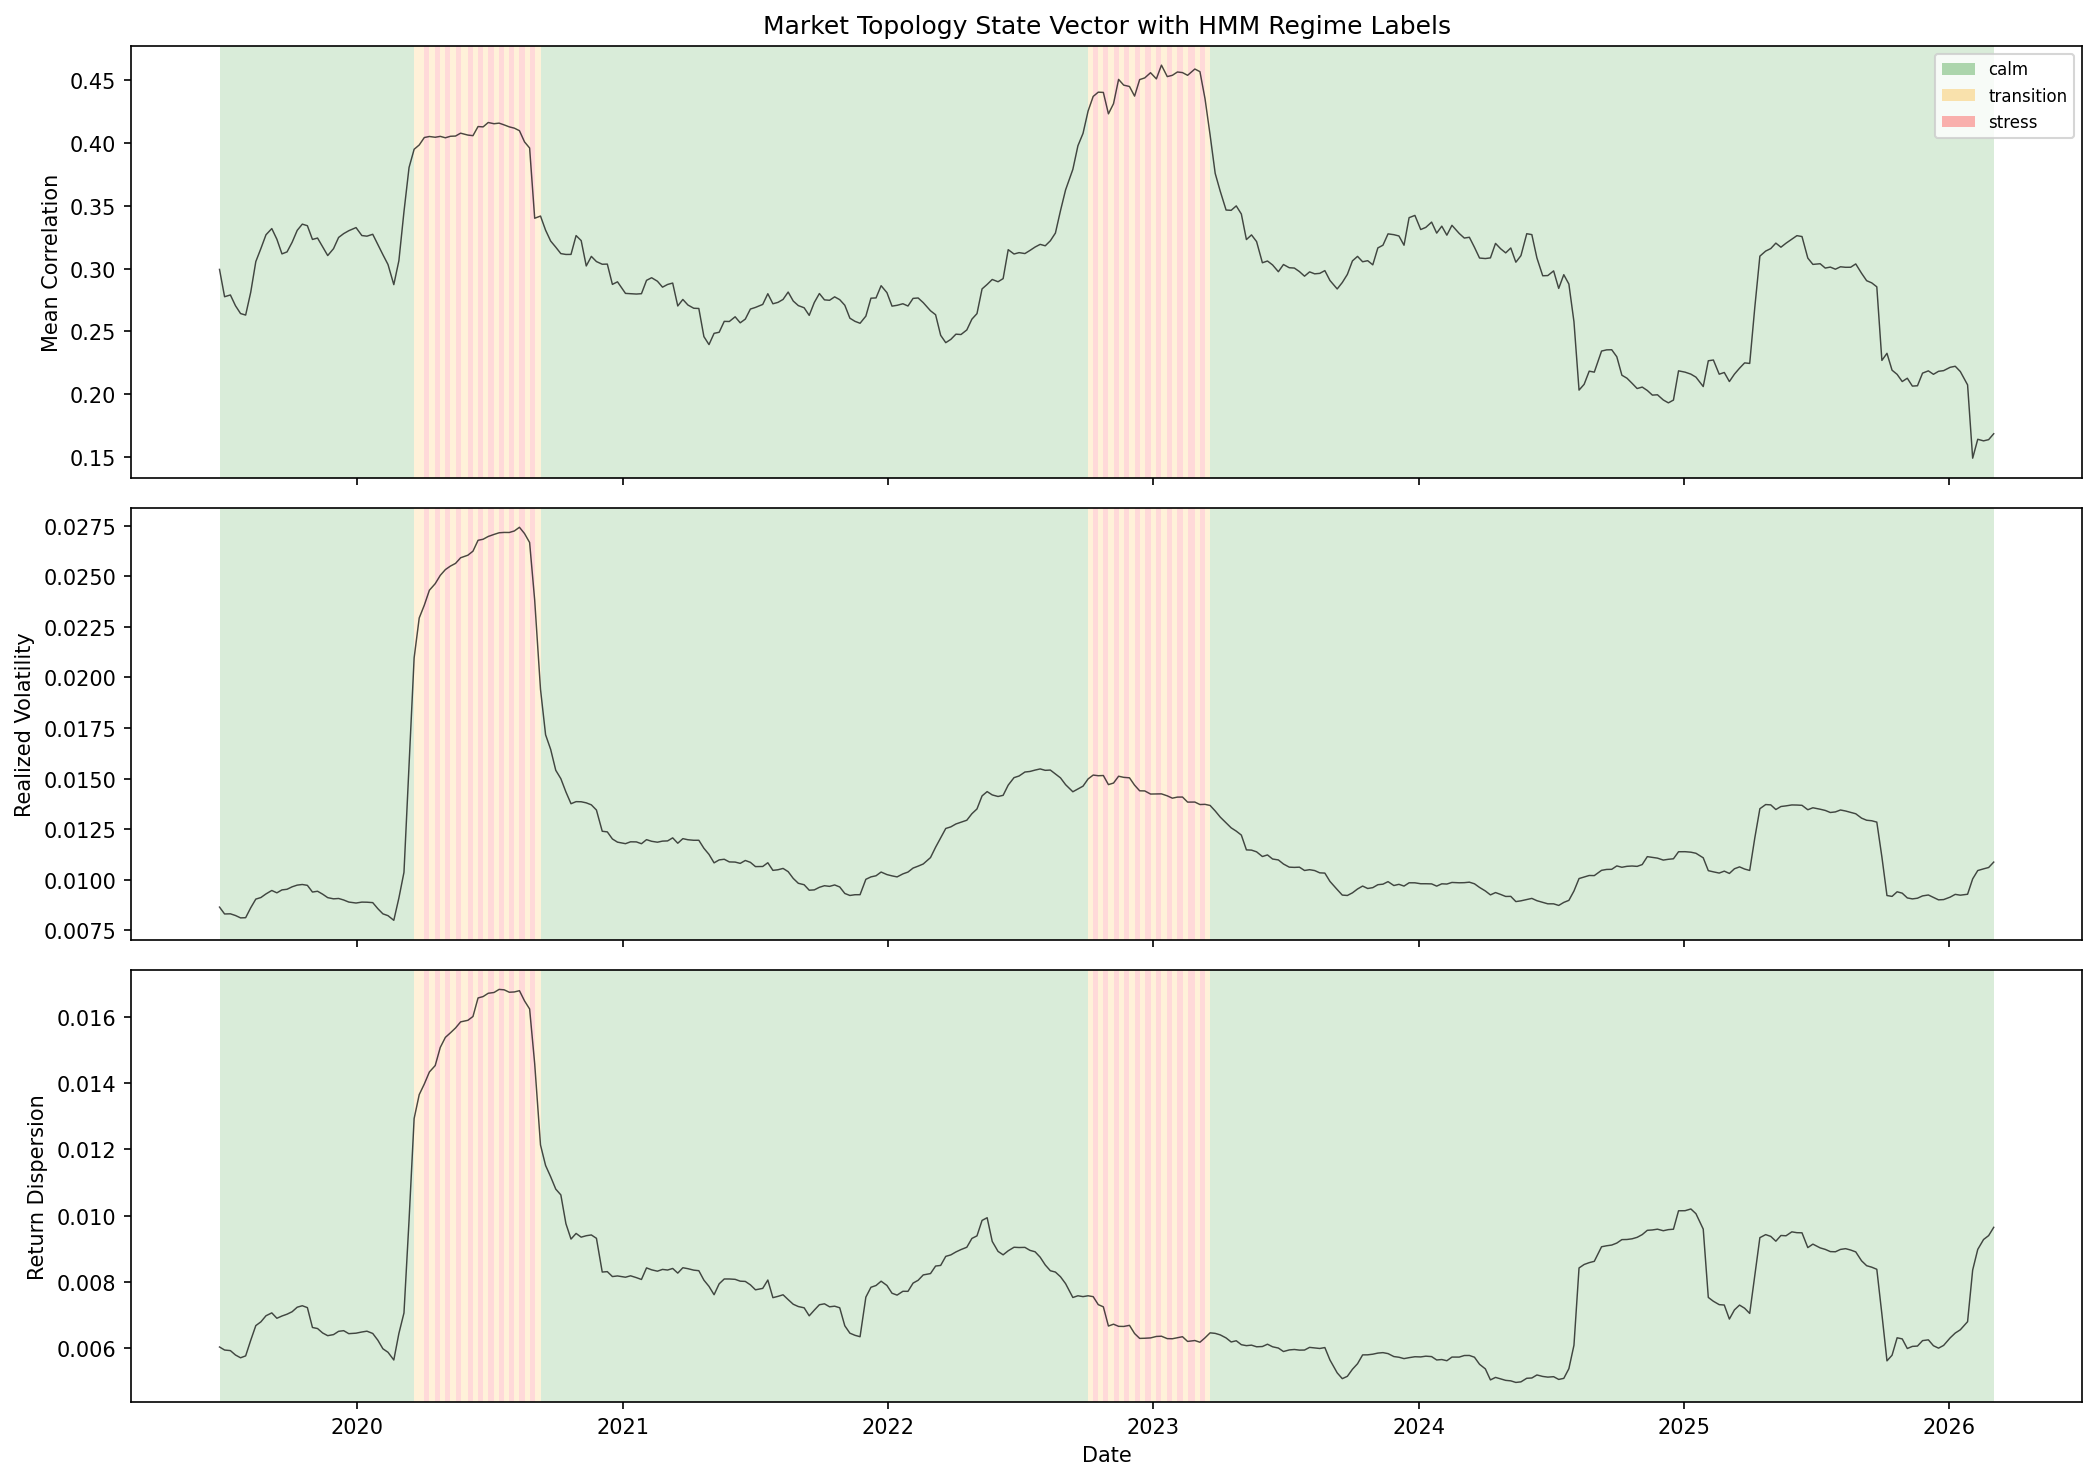
\includegraphics[width=\textwidth]{fig2_regime_detection.png}
\caption{HMM regime detection on the topology state vector. Three panels show mean correlation, realized volatility, and return dispersion with regime shading (green = calm, yellow = transition, red = stress).}
\label{fig:regime_detection}
\end{figure}

\subsection{Random Forest (Out-of-Sample Regime Validation)}

To make sure the HMM regimes are not just fitting noise, we validate them out-of-sample using a constrained Random Forest classifier. The input features are topology metrics (CMI, TDS, layer agreement, centrality statistics) and the target is the HMM-assigned regime label. We use TimeSeriesSplit for the cross-validation to prevent any look-ahead bias, and we constrain the tree depth and feature count to avoid overfitting.

This is not a regime prediction model in the forecasting sense. Its purpose is validation: if topology metrics can predict regime labels out-of-sample, that tells us the regimes correspond to genuinely different topological states rather than being artifacts of the HMM fitting process.

%----------------------------------------------------------------------
\section{Implementation and Results}
%----------------------------------------------------------------------

\subsection{Pipeline Architecture}

The full analysis runs as an 8-step CLI pipeline built with Typer for command dispatch and Rich for logging. The codebase totals roughly 6,200 lines of Python spread across 10 source directories, with 32 unit tests covering all core modules:

\begin{enumerate}
    \item \texttt{fetch-data}: pulls all universe tickers from FMP via async API calls
    \item \texttt{validate-data}: checks for staleness, coverage gaps, and missing data
    \item \texttt{build-features}: cleans and aligns prices, computes log returns, saves to parquet
    \item \texttt{run-clustering}: runs rolling-window Leiden across all 764 windows
    \item \texttt{run-regimes}: fits the 3-state Gaussian HMM on the topology feature vector
    \item \texttt{run-migration}: computes CMI, AMF, CPS, and TDS with full graph history
    \item \texttt{compute-centrality}: betweenness, eigenvector, degree, and closeness per window
    \item \texttt{export-topology}: writes 4 parquet files for downstream consumption
\end{enumerate}

\subsection{Novel Migration Metrics}

We developed four metrics for quantifying cluster migration over time. Each one addresses a gap in how existing literature handles temporal cluster comparisons.

\textbf{CMI (Cluster Migration Index)} measures the fraction of assets that genuinely changed cluster between consecutive windows:

\begin{equation}
    \text{CMI}(t) = \frac{1}{N} \sum_{i=1}^{N} \left[ 1 - \delta\!\left(\sigma\!\left(c_i(t)\right),\; c_i(t-1)\right) \right]
\end{equation}

where $\sigma$ is the Hungarian-optimal bijection \cite{kuhn1955} between label sets. Without this matching step, Leiden's arbitrary relabeling inflates CMI systematically.

\textbf{TDS (Topology Deformation Score)} captures graph-level structural change through three z-normalized components:

\begin{equation}
    \text{TDS}(t) = \alpha \cdot z\!\left(W_{\text{degree}}(t)\right) + \beta \cdot z\!\left(J_{\text{community}}(t)\right) + \gamma \cdot z\!\left(S_{\text{spectral}}(t)\right)
\end{equation}

where $W_{\text{degree}}$ is the Wasserstein-1 distance between degree distributions, $J_{\text{community}}$ is the NMI-based community divergence, and $S_{\text{spectral}}$ is the Wasserstein distance between Laplacian eigenvalue spectra.

\textbf{AMF (Asset Migration Frequency)} identifies which individual assets are most structurally unstable over time using per-step Hungarian matching. \textbf{CPS (Cluster Persistence Score)} measures how well specific clusters hold together via Hungarian-matched Jaccard overlap.

\subsection{Directional Information Flow}

Net transfer entropy via the KSG estimator gives us a directed measure of who leads and who follows:

\begin{equation}
    \text{NTE}(X \to Y) = \text{TE}(X \to Y) - \text{TE}(Y \to X)
\end{equation}

We also test cross-layer Granger causality: whether tail-dependence CMI predicts Pearson CMI. The result ($p = 0.041$) is significant, meaning the crash structure reshuffles before correlation catches up.

\subsection{Preliminary Results}

\begin{table}[H]
\centering
\caption{Full Pipeline Results (v0.5.0, January 2010 to March 2026)}
\begin{tabular}{@{}ll@{}}
\toprule
\textbf{Metric} & \textbf{Value} \\
\midrule
Assets surviving cleaning & 59 of 96 \\
Trading days & 3,938 \\
Rolling windows & 764 (120-day, 5-day step) \\
Active clusters (latest window) & 6 \\
HMM regimes & 3: calm (89.7\%), transition (5.1\%), stress (5.2\%) \\
Current regime (2026-03-20) & \textbf{STRESS} \\
Mean CMI & 0.094 \\
Max CMI & 0.441 \\
Mean TDS & 0.022 \\
Max TDS & 10.195 \\
\bottomrule
\end{tabular}
\end{table}

Figure~\ref{fig:cmi_tds} shows CMI and TDS over the full sample period with event windows highlighted. The COVID spike (blue shading, 2020) shows CMI hitting near 1.0, meaning total cluster dissolution. The Iran-Israel events (red and yellow shading, 2024-2025) show elevated but more sustained structural change. The key pattern across all events: topology deformation often precedes the acute shock.

\begin{figure}[H]
\centering
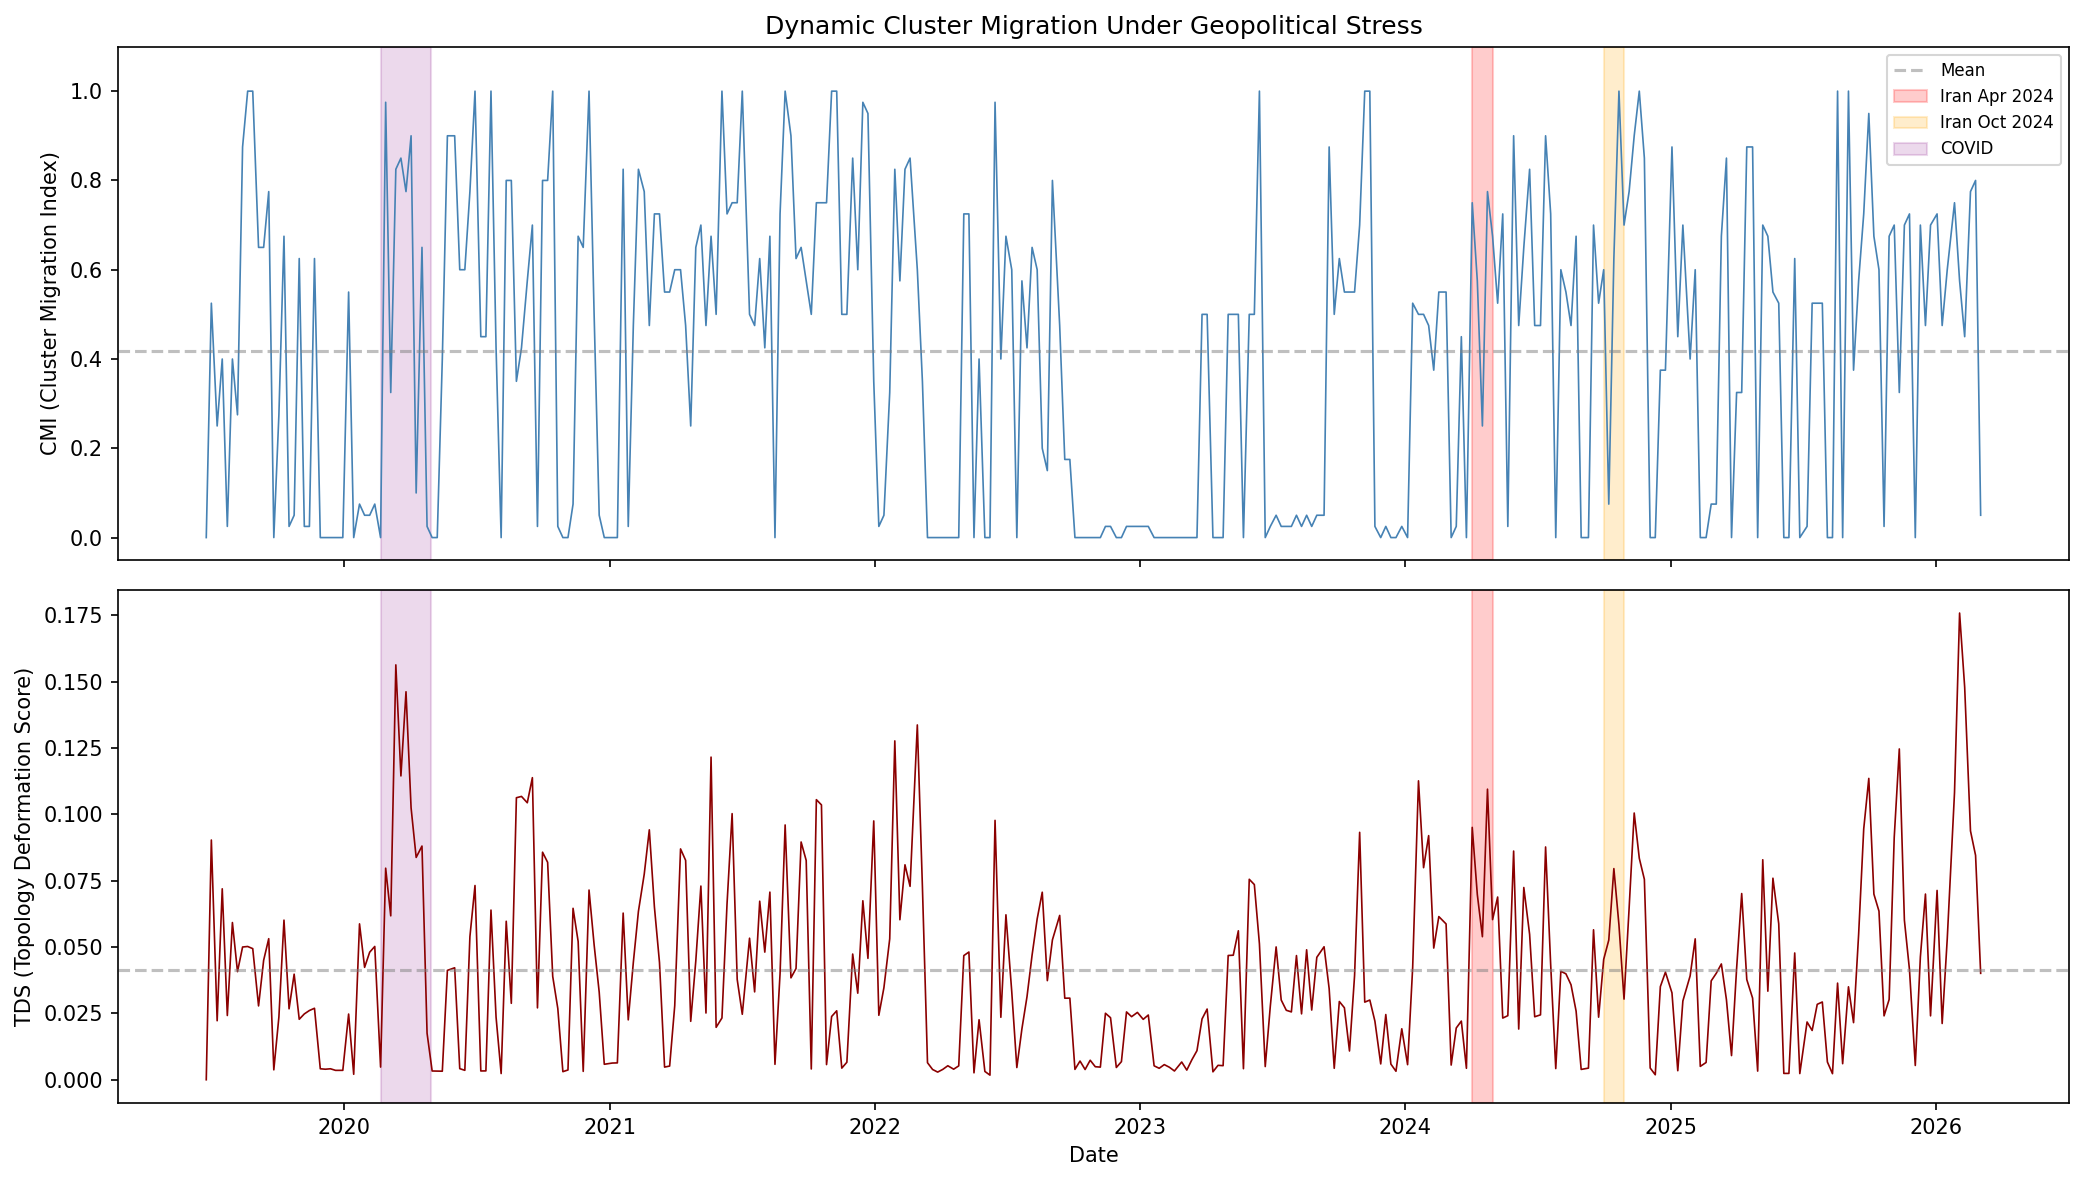
\includegraphics[width=\textwidth]{fig1_cmi_tds_timeseries.png}
\caption{CMI (top) and TDS (bottom) over the full sample with geopolitical event windows shaded. Dashed lines indicate mean values. Note the pre-event elevation in TDS before several of the shaded crisis windows.}
\label{fig:cmi_tds}
\end{figure}

Figure~\ref{fig:amf_bar} ranks all assets by their migration frequency. EWZ (Brazil), UUP (Dollar), and FXE (Euro) are the most migratory, while IWM, XLI, and other core US equities are the most stable. Commodity and FX assets dominate the high-migration end, which tracks with their exposure to idiosyncratic supply-side and geopolitical shocks.

\begin{figure}[H]
\centering
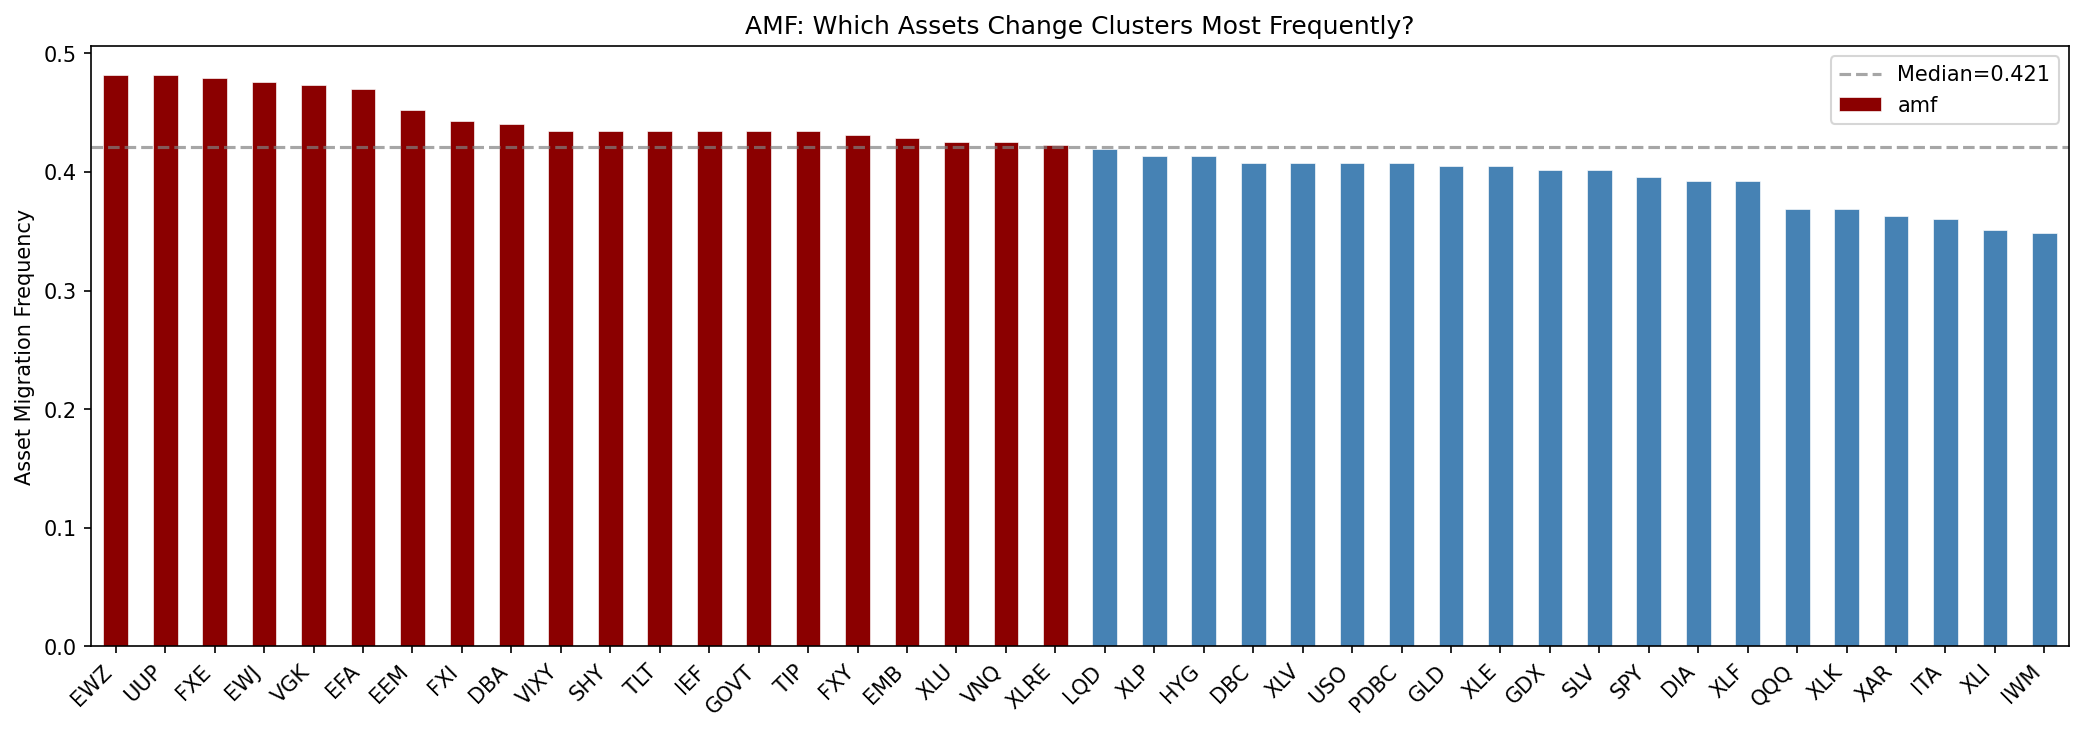
\includegraphics[width=\textwidth]{fig5_amf_bar.png}
\caption{Asset Migration Frequency ranking across the full sample. Red bars indicate assets above the median migration rate. EM and commodity assets dominate the high end; core US equity clusters at the low end.}
\label{fig:amf_bar}
\end{figure}

Figure~\ref{fig:info_flow} shows the net transfer entropy ranking, answering the question of who leads and who follows in the information flow network. HYG (high yield credit) is the top net sender with +0.385, followed by SHY and EEM. FXE (euro) is the largest net receiver at -0.529. This ranking flips during stress regimes, when Treasuries take over as the primary senders.

\begin{figure}[H]
\centering
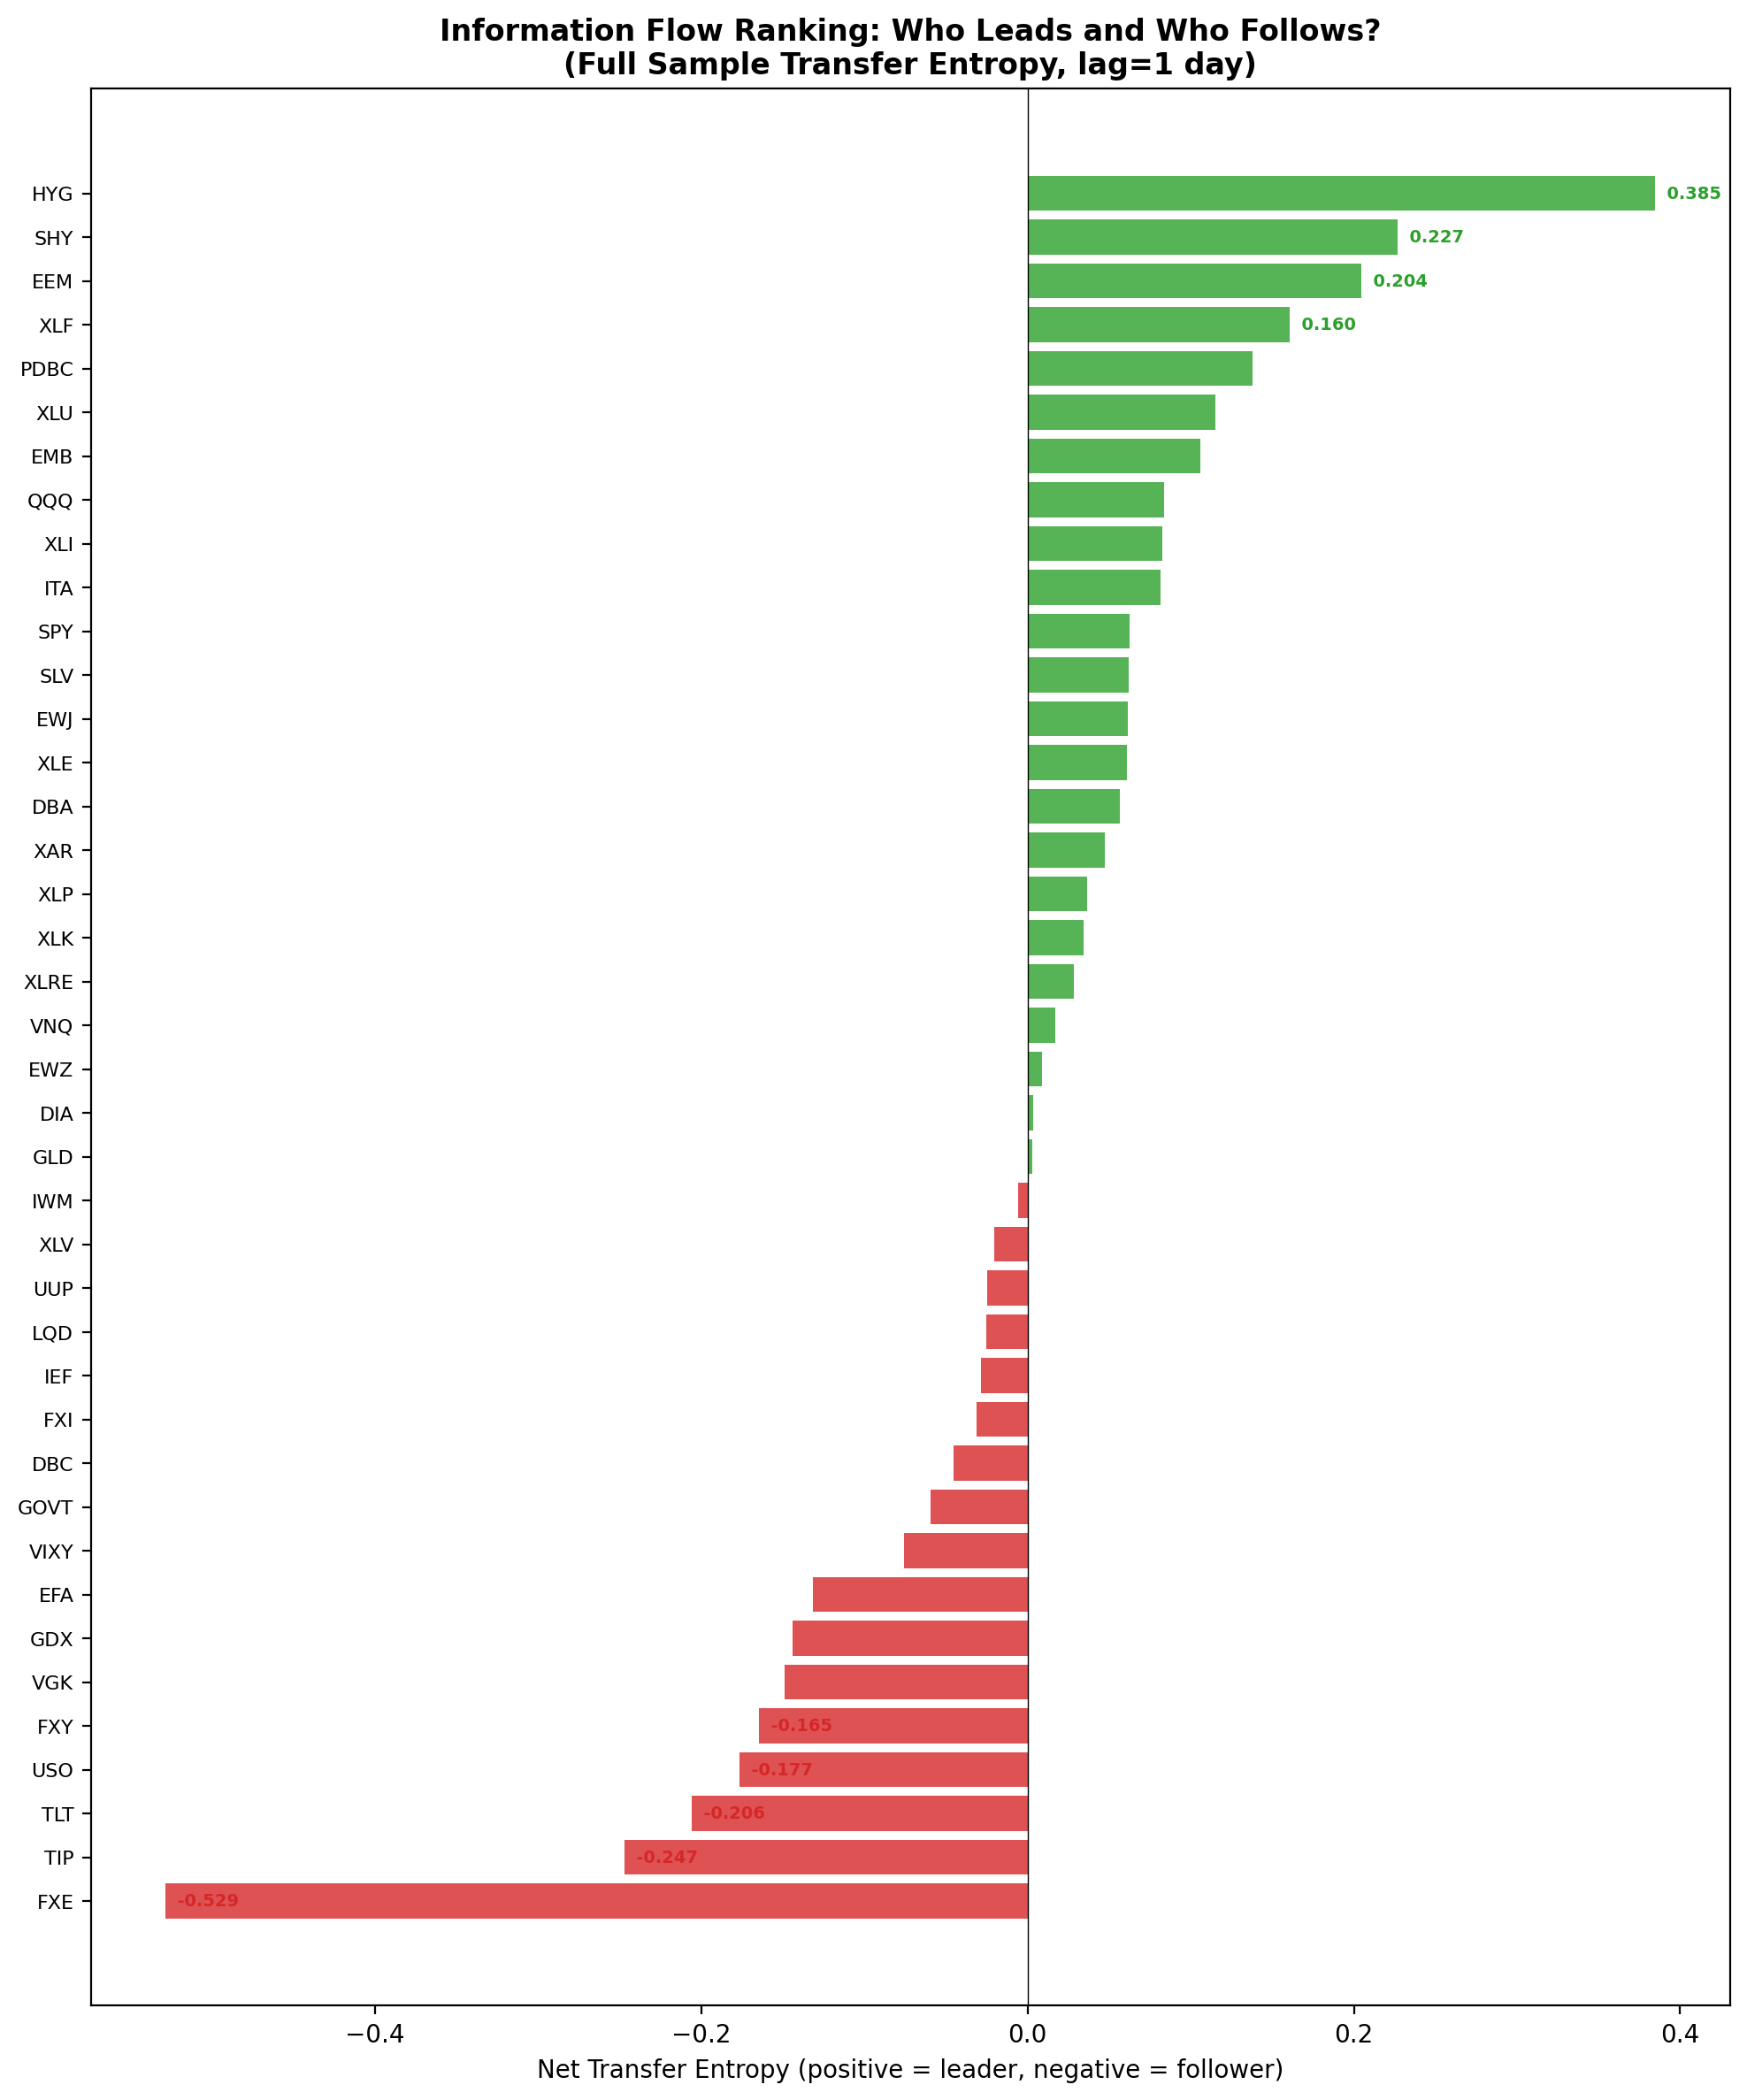
\includegraphics[width=\textwidth]{fig13_information_flow_ranking.png}
\caption{Net transfer entropy ranking across all assets. Green = net information sender (leader), red = net information receiver (follower). HYG leads overall; FXE is the largest receiver.}
\label{fig:info_flow}
\end{figure}

Figure~\ref{fig:cross_layer_granger} shows the cross-layer Granger causality results. Only one direction is significant: Tail $\to$ Pearson ($F = 2.78$, $p = 0.041$). All other layer-pair directions fall below the significance threshold. This confirms that structural change in the extreme co-movement layer leads structural change in the linear correlation layer.

\begin{figure}[H]
\centering
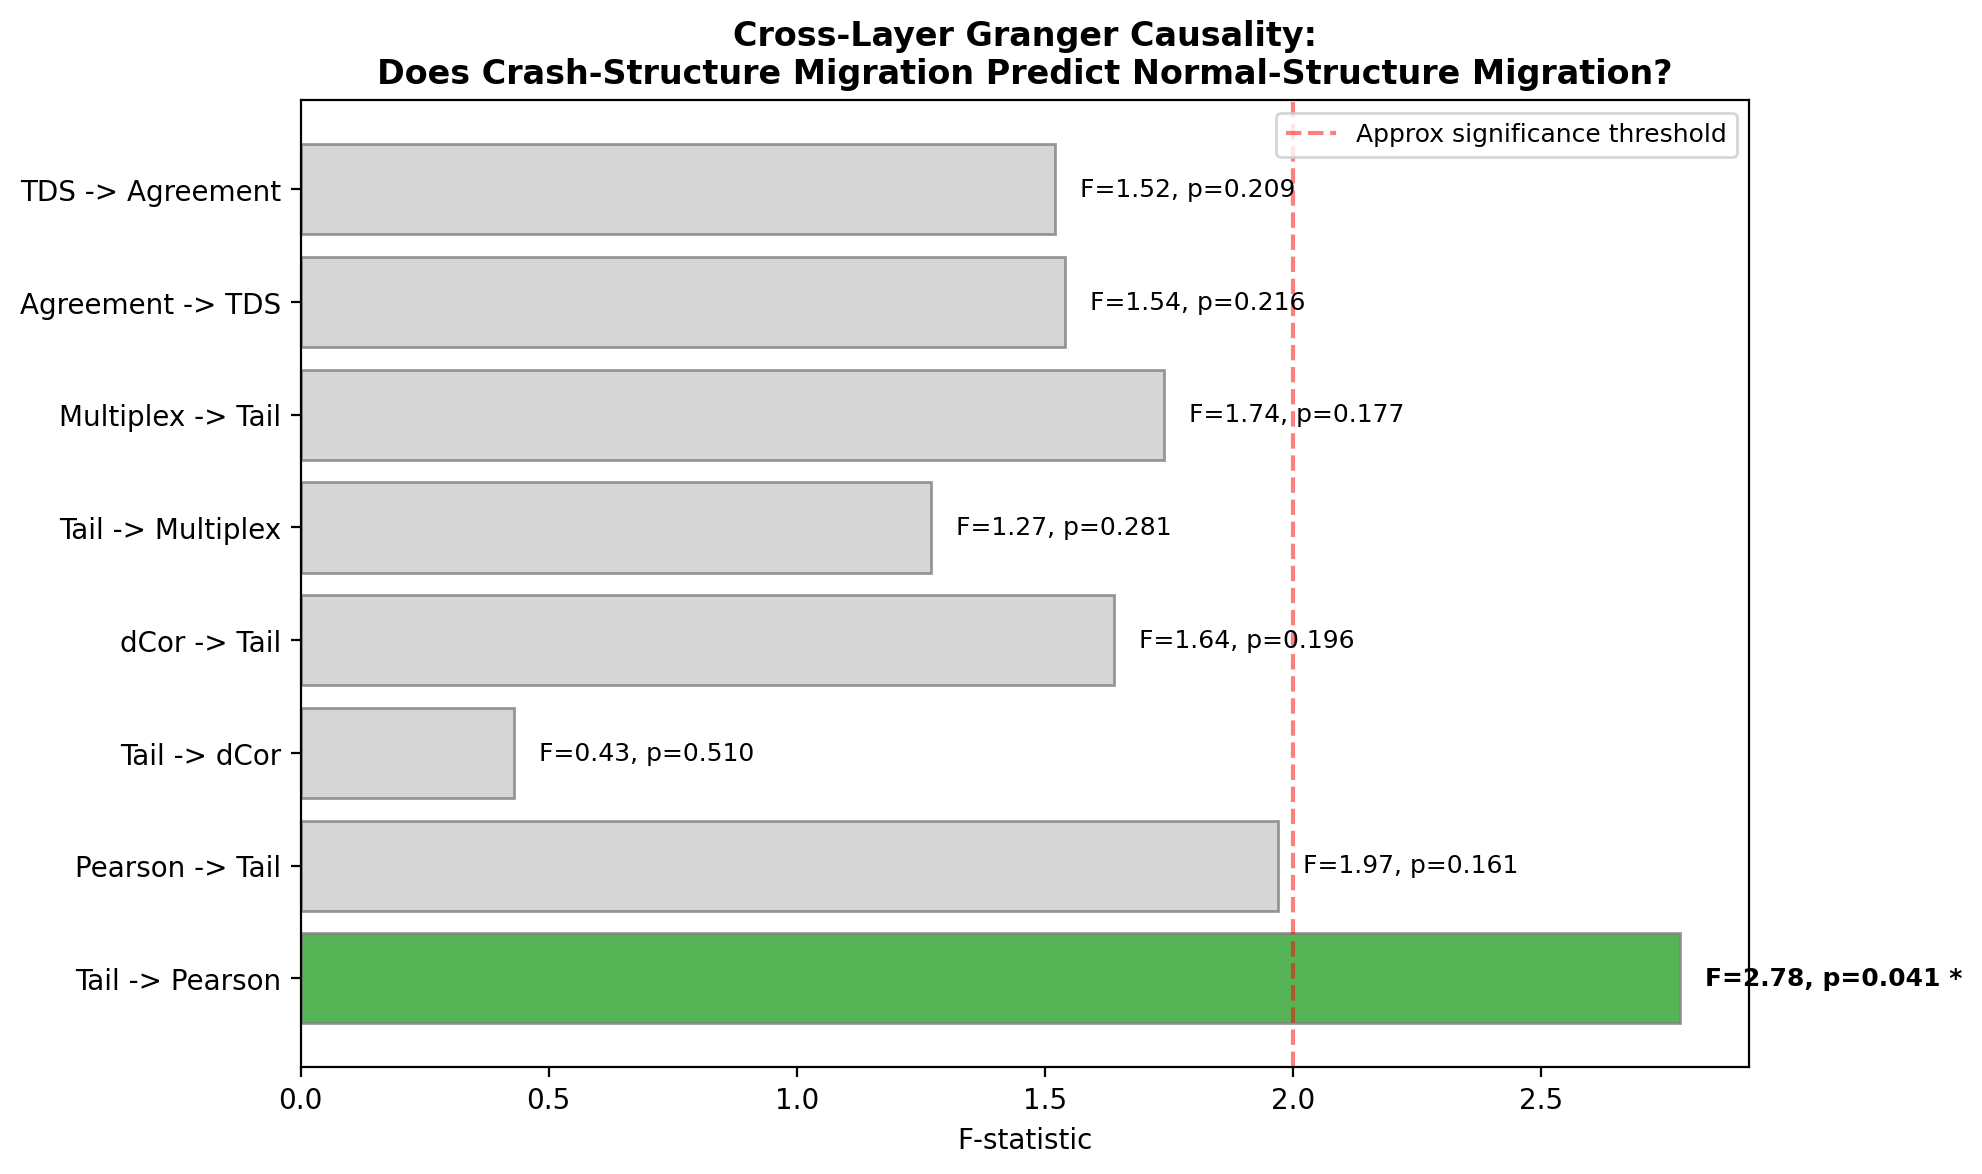
\includegraphics[width=\textwidth]{fig17_cross_layer_granger.png}
\caption{Cross-layer Granger causality F-statistics. Only the Tail $\to$ Pearson direction exceeds the significance threshold (dashed red), with $p = 0.041$.}
\label{fig:cross_layer_granger}
\end{figure}

Figure~\ref{fig:covid_evolution} shows the COVID-19 cluster evolution across four phases: pre-COVID baseline, early spread, market crash, and recovery rally. During the crash phase, the clear 4-cluster baseline structure dissolves and reforms with different membership. The recovery rally shows a new 6-cluster structure that is noticeably different from the pre-COVID configuration.

\begin{figure}[H]
\centering
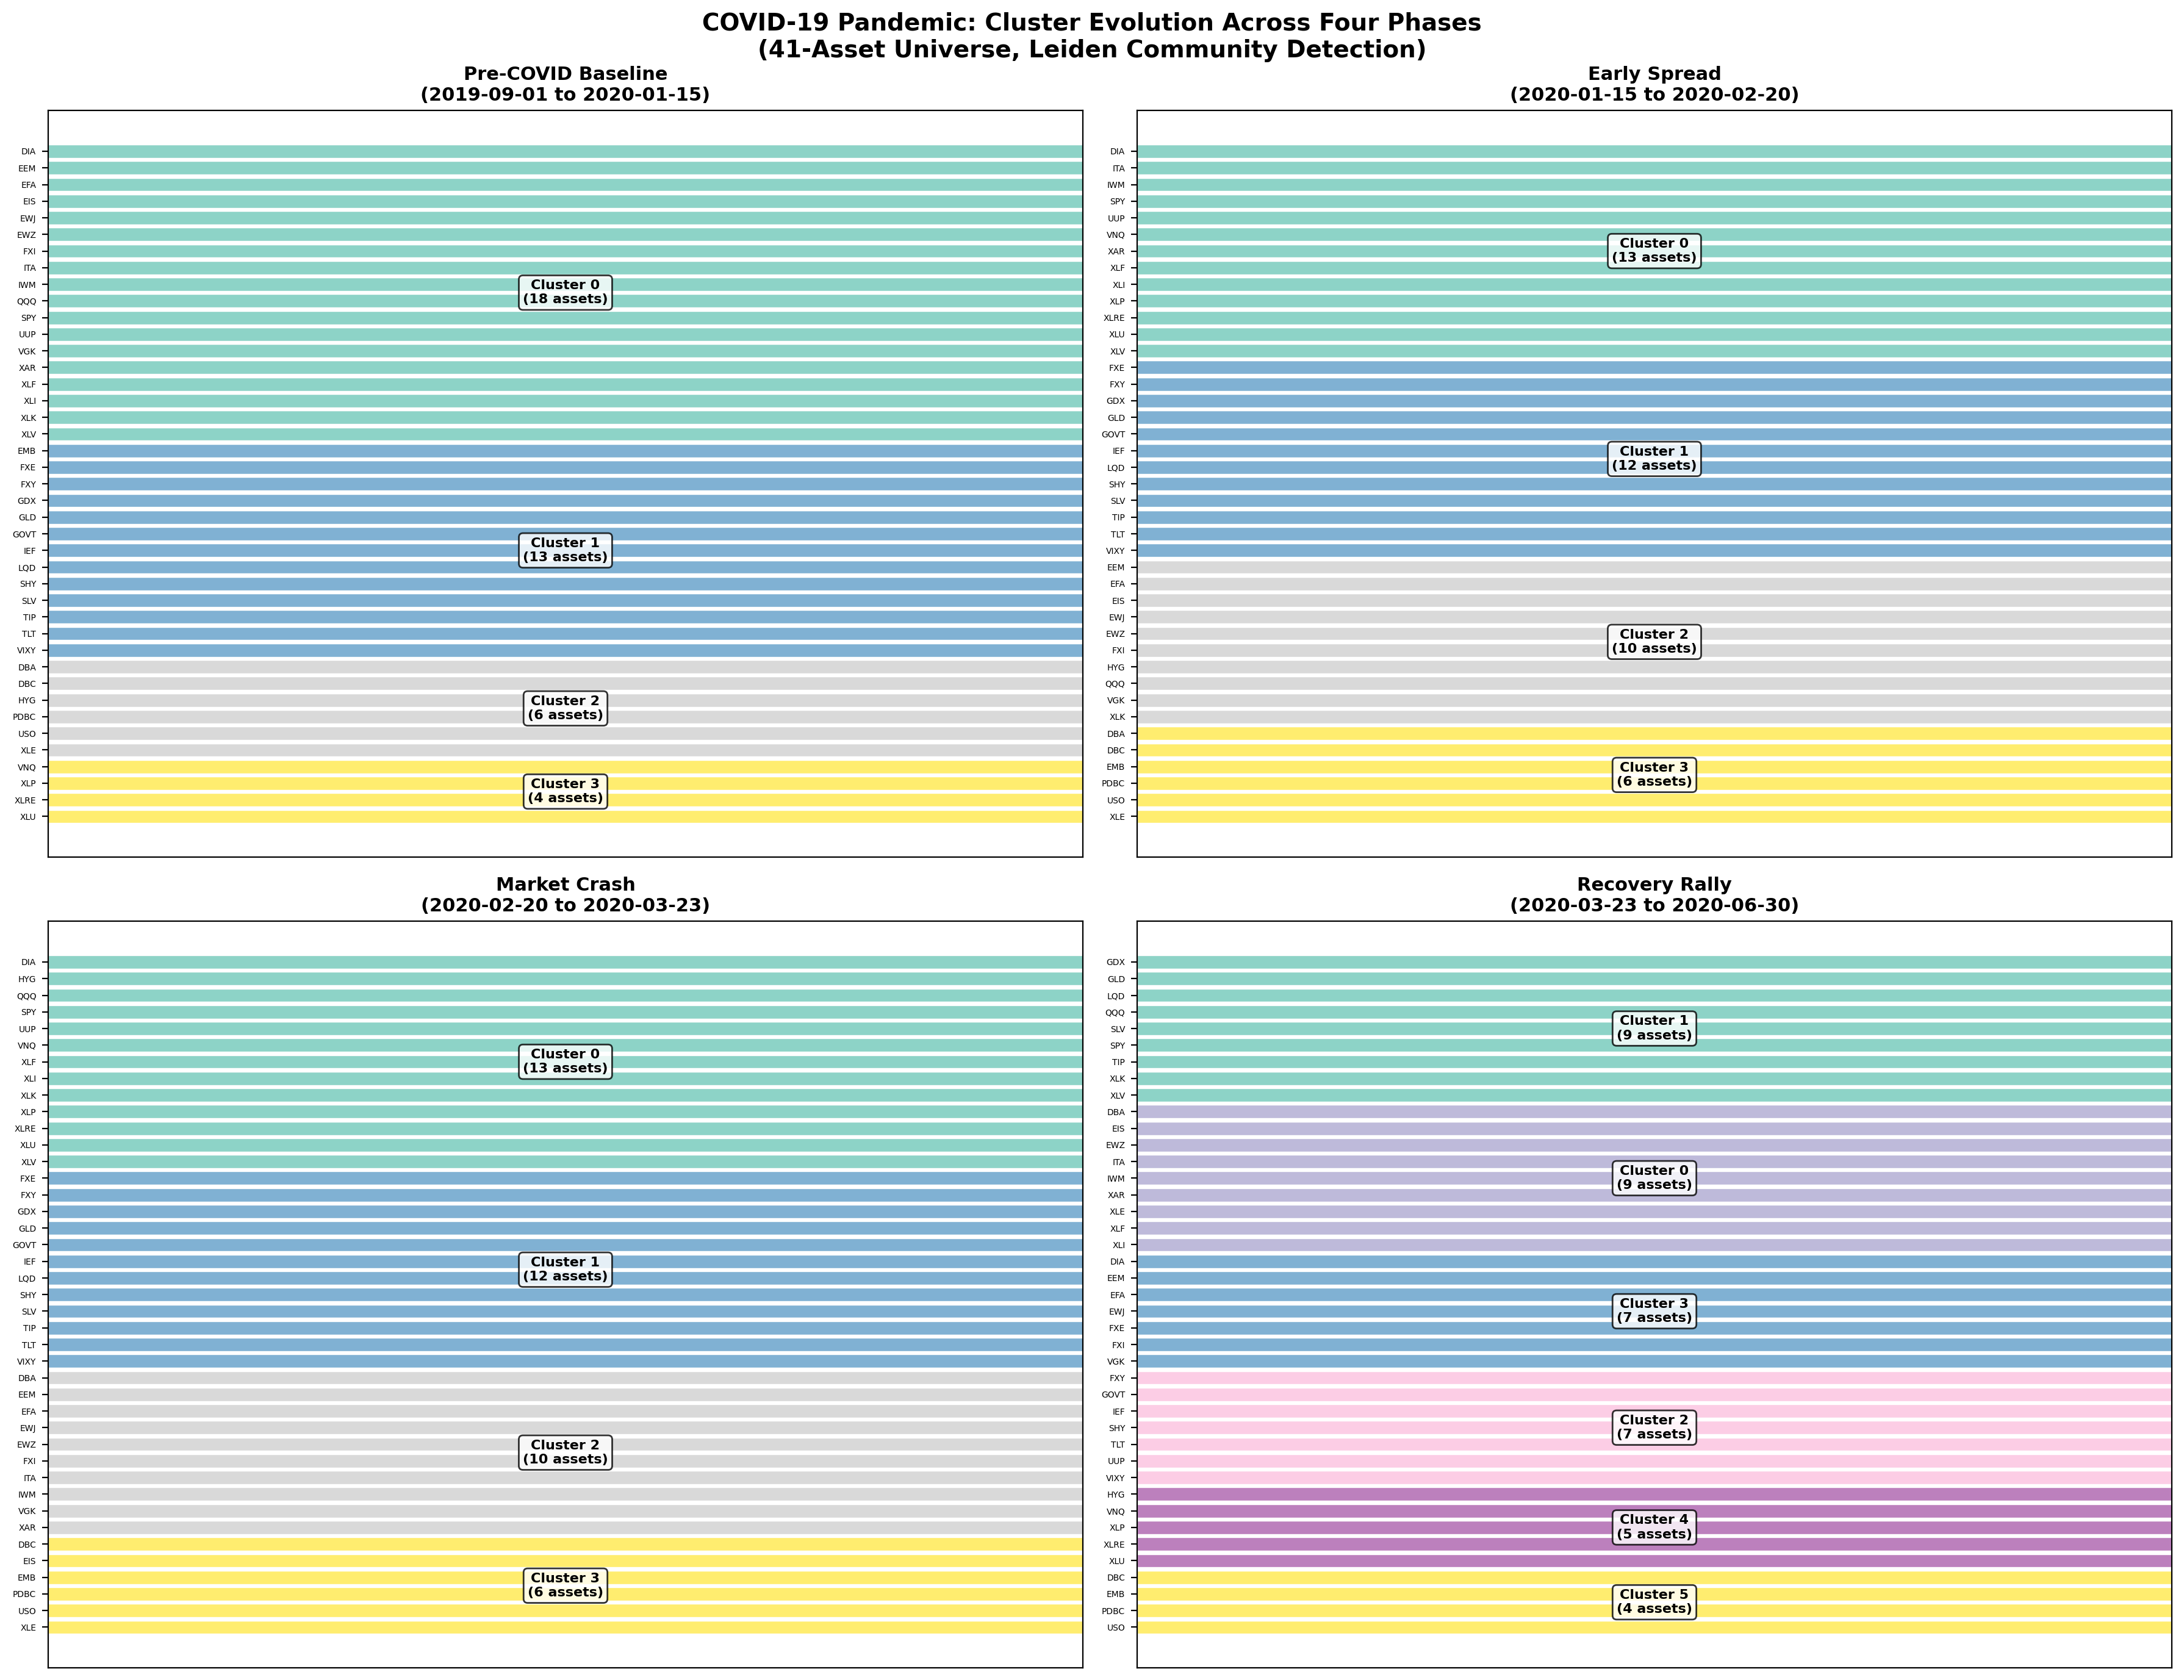
\includegraphics[width=\textwidth]{fig18_covid_cluster_evolution.png}
\caption{COVID-19 cluster evolution across four phases. Each colored band represents a different cluster. Notice the complete restructuring during the crash phase and the emergence of new clusters during recovery.}
\label{fig:covid_evolution}
\end{figure}

\subsection{Topology Export}

The pipeline exports four parquet files designed for reproducibility and integration with downstream ML work:

\begin{itemize}
    \item \texttt{cluster\_membership.parquet}: 45,076 rows covering date, ticker, cluster ID, days since last migration, and cluster size
    \item \texttt{centrality\_metrics.parquet}: 45,076 rows with degree, betweenness, eigenvector, and closeness centrality per asset per window
    \item \texttt{regime\_states.parquet}: 3,918 rows with regime label, probability, and persistence count
    \item \texttt{topology\_deformation.parquet}: 763 rows with TDS score, TDS z-score, and layer agreement
\end{itemize}

%----------------------------------------------------------------------
\section{Event Studies}
%----------------------------------------------------------------------

We defined 8 geopolitical event windows across the 16-year dataset, each subdivided into pre-event calibration, escalation buildup, acute shock, counter-response, digestion, and normalization phases. The sub-windowing matters because it lets us track how topology evolves through the full lifecycle of a crisis, rather than just capturing the spike.

The events, in chronological order:

\begin{enumerate}
    \item European Sovereign Debt Crisis and US Downgrade (2011)
    \item COVID-19 Market Crash (March 2020)
    \item Fed Hawkish Repricing (2022)
    \item SVB Banking Stress (March 2023)
    \item Iran-Israel, April 2024 (Operation True Promise I)
    \item Japan Carry Trade Unwind (August 2024)
    \item Iran-Israel, October 2024 (Operation True Promise II)
    \item DeepSeek AI Cost Shock (January 2025)
\end{enumerate}

\subsection{Iran-Israel Conflict Cycle}

This is our primary case study, and it is ideal for our purposes because it spans three distinct escalation events over 14 months, each producing a different market response.

In April 2024 (True Promise I), Iran launched over 170 drones, 30 cruise missiles, and 120 ballistic missiles at Israel on April 13-14, the first direct military exchange between the two countries. What we observed in the topology data was that the restructuring began during the buildup phase from April 1-12, \textit{before} the actual strikes. By the time the missiles flew, the market had already repositioned itself structurally.

October 2024 (True Promise II) saw approximately 180 ballistic missiles launched on October 1. Israel's counter-strike on October 26 deliberately avoided oil infrastructure. Oil crashed 5-6\% on that news, not because the strike was bad, but because the market had priced in something much worse and the restraint triggered a relief unwind.

The June 2025 escalation (Operation Epic Fury / Twelve-Day War) produced our highest TDS reading: 0.176, which actually exceeded COVID. And here is what made it so striking: the Pearson correlation layer showed almost nothing. If we had been running a single-layer analysis, we would have missed the entire structural event. The dCor and tail-dependence layers, however, picked up massive and sustained restructuring. This event alone justified the multi-layer design.

\subsection{COVID-19}

COVID remains the most extreme single-window reading in our dataset: CMI of 1.0. Every single asset changed cluster assignment in a single step. Complete topological dissolution, as shown in Figure~\ref{fig:covid_evolution}. But the recovery was surprisingly fast. Within a few weeks, recognizable community structure had re-formed, and the new structure was not radically different from pre-COVID.

Compare that to the geopolitical shocks, which tend to produce lower peak CMI values but much longer-lasting asymmetric shifts. The topology does not snap back the way it does after a symmetric shock like a pandemic selloff. The driving forces (sanctions, conflict, supply chain disruption) persist, and so does the structural change.

%----------------------------------------------------------------------
\section{Key Findings}
%----------------------------------------------------------------------

\subsection{Pre-Event Restructuring}

The finding we kept seeing across events, and the one we consider most significant, is that markets restructure before the geopolitical event, not during it. Peak topology deformation during the Iran-Israel cycle happened in the buildup to Operation Epic Fury, not when strikes were actually underway. The network was already in its stressed configuration by the time the news broke.

Volatility tells you the event happened. That is useful, but it is retrospective. What the topology data shows is that the repositioning was already underway days before the strikes, which is a different kind of information entirely and arguably the more useful one.

\subsection{Multi-Layer Necessity}

The June 2025 Twelve-Day War was invisible to Pearson correlation. This is the strongest argument for the multi-layer design in our entire dataset. A single-layer Pearson analysis would have produced a qualitatively wrong conclusion about one of the most significant geopolitical escalations in the sample. The dCor layer picked it up. The tail-dependence layer picked it up even more clearly. But Pearson? Nothing. That is not a theoretical concern about methodology. That is a real event in real data where the standard approach fails completely.

\subsection{Cross-Layer Causality}

The tail-dependence CMI Granger-causes the Pearson CMI at $p = 0.041$ (Figure~\ref{fig:cross_layer_granger}). In plain terms, the crash structure reshuffles first and the normal-conditions correlation catches up later. That is exactly the ordering you would want if you were trying to build an early warning system out of this: monitor the tail-dependence CMI, and if it starts spiking while Pearson CMI is still flat, correlation structure is probably about to shift.

\subsection{Regime-Dependent Leadership}

Transfer entropy analysis revealed that the direction of information flow between assets flips depending on the market regime (Figure~\ref{fig:info_flow}). During calm periods, credit instruments (HYG in particular) and real estate assets tend to lead information flow. During war and stress regimes, the Treasury complex (TLT, GOVT, TIP) takes over as the primary sender.

Credit spreads have always been a leading indicator of risk appetite in practice, so seeing HYG dominate net TE is consistent with that. FXE sitting on the receiving end makes sense too, since the euro tends to absorb global risk spillover from pretty much everywhere.

\subsection{Migration Characteristics by Asset Class}

Commodity and frontier emerging market assets consistently show the highest migration frequencies (Figure~\ref{fig:amf_bar}). They sit at the edges of the cluster structure and periodically get pulled into different groups depending on the macro regime. Core US large-cap equity almost never changes cluster assignment. It is structurally anchored.

Fixed income plays a different role entirely. EMB (emerging market bonds) and SHY (short-term Treasuries) have the highest betweenness centrality in the network, meaning they sit on the shortest paths between other clusters more than anything else. They are not the ones migrating, but they are the connective tissue holding the structure together. We did not expect SHY to rank that high, honestly. You would think short-duration Treasuries would be too boring to matter in a network sense, but their role as a parking asset during flight-to-quality flows puts them at the crossroads of everything.

EEM (MSCI Emerging Markets) comes out as the most central asset overall across degree, eigenvector, and closeness centrality. Not surprising, given that EM equity touches essentially everything: commodities through resource exporters, currencies through EM FX, US equities through risk appetite, fixed income through EM spreads. It ends up acting as a hub that amplifies shocks no matter which direction they come from.

%----------------------------------------------------------------------
\section{Methodological Corrections}
%----------------------------------------------------------------------

We want to be upfront about the issues we discovered and fixed during development. Some of these are common pitfalls in the financial networks literature, and documenting them felt important.

\textbf{CMI permutation invariance.} The biggest one. Without Hungarian matching, every time Leiden relabeled clusters (which it does constantly since labels are arbitrary), the CMI metric counted that as real migration. Our fix uses \texttt{scipy.optimize.linear\_sum\_assignment} to find the optimal label bijection before computing migration.

\textbf{TDS component incommensurability.} The three TDS components have completely different natural scales. Combining them without normalization is like adding meters to kilograms. The \texttt{TDSNormalizer} class maintains running z-scores for each component so the weighted sum is actually meaningful.

\textbf{Spectral distance on varying graph sizes.} Zero-padded $L_2$ norm on Laplacian eigenvalues breaks when graphs have different numbers of nodes across windows. Wasserstein distance between eigenvalue distributions handles varying lengths naturally.

\textbf{MST edge weight double-counting.} Summing upper and lower triangles of a symmetric similarity matrix doubles every weight. Small bug, real impact on tree structure. Fixed to take max of symmetric entries.

\textbf{Granger causality lag selection.} Testing multiple lag specifications and selecting the minimum $p$-value is textbook $p$-hacking. We apply Bonferroni correction across all tested lags before selecting the best one.

\textbf{Granger on non-stationary series.} Running Granger causality on non-stationary time series produces spurious results. We added an ADF stationarity pre-check; any pair that fails stationarity gets flagged with $p=1.0$ rather than producing a misleading significant result.

\textbf{PELT change-point over-detection.} The original penalty formula ($\log(n) \cdot \text{Var}(x)$) was too lenient and flagged too many changepoints. Switching to proper BIC ($d \cdot \log(n)$ with $d=2$) resolved this.

%----------------------------------------------------------------------
\section{Roadmap and Future Work}
%----------------------------------------------------------------------

The framework as it stands is complete through Phase 5. There are several directions we want to take it.

\subsection{Real-Time Extension (Phase 6)}

The most natural next step is moving from batch analysis to real-time monitoring. We want a streaming data pipeline that updates rolling windows incrementally, a live dashboard (probably Streamlit or Dash) that tracks CMI, TDS, and layer agreement as they evolve, and an alert system for when tail CMI spikes or TE leadership patterns flip. The pipeline architecture already supports most of this. The streaming ingestion is the straightforward part. The harder problem is computing rolling dependency matrices incrementally without reprocessing the entire window from scratch every time new data comes in.

\subsection{Extended Research (Phase 7)}

Several extensions would strengthen the research:

\begin{itemize}
    \item Extending the dataset back to the 2008 Global Financial Crisis using ETFs available from that era
    \item Incorporating intraday 5-minute returns during crisis windows to see within-day topology evolution
    \item Applying more rigorous causal discovery methods like PCMCI+ or DYNOTEARS
    \item Adding a geopolitical NLP layer that ingests GDELT event data or news embeddings as an exogenous signal
    \item A deeper analysis of crypto assets (BTC, ETH, SOL, DeFi indices) as they become a larger part of the cross-asset landscape
\end{itemize}

\subsection{Robustness Completion}

The Phase 4 statistical robustness framework is fully implemented and unit-tested, but running it end-to-end on the complete 96-ETF dataset is still pending. The computational cost is significant: 1,000 bootstrap resamples across 764 windows, multiplied by the pairwise test counts. This will likely need dedicated batch compute time rather than running on a local machine.

%----------------------------------------------------------------------
\section{Conclusion}
%----------------------------------------------------------------------

When we started this project, we assumed the main value would be in the multi-layer design itself. And it was. But the finding we did not expect was how consistently tail dependence leads linear correlation across completely different types of events, from a pandemic selloff to a Middle Eastern escalation to an AI cost shock. That ordering showed up everywhere, and it ended up being the result with the most practical relevance.

The methodological corrections also turned out to be more important than we initially thought. Hungarian matching for CMI sounds like a minor implementation detail until you realize that without it, your migration readings are systematically inflated across the entire time series. Same story with TDS normalization. These are not edge cases. They change the quantitative results on real data, and the fact that they are rarely addressed in the existing financial networks literature suggests that a lot of published migration analysis may be noisier than it needs to be.

If there is one takeaway from 16 years of data and 8 geopolitical events, it is that watching correlation alone means you are always a step behind. The topology moves first. The tails tell you it is coming. By the time Pearson catches up, the structural shift already happened.

The codebase is open-source and reproducible from a single CLI command. The topology export is designed to plug directly into downstream ML work, which is where we plan to take this next.

%----------------------------------------------------------------------
% References
%----------------------------------------------------------------------
\bibliographystyle{plain}
\begin{thebibliography}{20}

\bibitem{szekely2007}
G.~J. Sz\'{e}kely, M.~L. Rizzo, and N.~K. Bakirov.
\newblock Measuring and testing dependence by correlation of distances.
\newblock \textit{The Annals of Statistics}, 35(6):2769--2794, 2007.

\bibitem{ledoit2004}
O.~Ledoit and M.~Wolf.
\newblock A well-conditioned estimator for large-dimensional covariance matrices.
\newblock \textit{Journal of Multivariate Analysis}, 88(2):365--411, 2004.

\bibitem{traag2019}
V.~A. Traag, L.~Waltman, and N.~J. van Eck.
\newblock From Louvain to Leiden: guaranteeing well-connected communities.
\newblock \textit{Scientific Reports}, 9(1):5233, 2019.

\bibitem{politis1992}
D.~N. Politis and J.~P. Romano.
\newblock A circular block-resampling procedure for stationary data.
\newblock In \textit{Exploring the Limits of Bootstrap}, pages 263--270. Wiley, 1992.

\bibitem{theiler1992}
J.~Theiler, S.~Eubank, A.~Longtin, B.~Galdrikian, and J.~D. Farmer.
\newblock Testing for nonlinearity in time series: the method of surrogate data.
\newblock \textit{Physica D}, 58(1-4):77--94, 1992.

\bibitem{schreiber1996}
T.~Schreiber and A.~Schmitz.
\newblock Improved surrogate data for nonlinearity tests.
\newblock \textit{Physical Review Letters}, 77(4):635, 1996.

\bibitem{storey2002}
J.~D. Storey.
\newblock A direct approach to false discovery rates.
\newblock \textit{Journal of the Royal Statistical Society: Series B}, 64(3):479--498, 2002.

\bibitem{benjamini1995}
Y.~Benjamini and Y.~Hochberg.
\newblock Controlling the false discovery rate: a practical and powerful approach to multiple testing.
\newblock \textit{Journal of the Royal Statistical Society: Series B}, 57(1):289--300, 1995.

\bibitem{kraskov2004}
A.~Kraskov, H.~St\"{o}gbauer, and P.~Grassberger.
\newblock Estimating mutual information.
\newblock \textit{Physical Review E}, 69(6):066138, 2004.

\bibitem{tumminello2005}
M.~Tumminello, T.~Aste, T.~Di~Matteo, and R.~N. Mantegna.
\newblock A tool for filtering information in complex systems.
\newblock \textit{Proceedings of the National Academy of Sciences}, 102(30):10421--10426, 2005.

\bibitem{mantegna1999}
R.~N. Mantegna.
\newblock Hierarchical structure in financial markets.
\newblock \textit{The European Physical Journal B}, 11(1):193--197, 1999.

\bibitem{kuhn1955}
H.~W. Kuhn.
\newblock The Hungarian method for the assignment problem.
\newblock \textit{Naval Research Logistics Quarterly}, 2(1-2):83--97, 1955.

\end{thebibliography}

%----------------------------------------------------------------------
% Disclaimer
%----------------------------------------------------------------------
\vspace{1em}
\noindent\rule{\textwidth}{0.4pt}
\small
\textbf{Disclaimer:} This document is produced solely for educational and academic research purposes as part of CPE 595 coursework at Stevens Institute of Technology. Nothing herein constitutes investment advice, a solicitation, or a recommendation to buy, sell, or hold any security or financial instrument. Past performance and historical patterns do not guarantee future results.

\end{document}
